\documentclass[11pt,a4paper]{book}

%\usepackage[scibook, thm, tikz, bib, index]{pmtex}

\PassOptionsToPackage{force}{filehook}
\usepackage{standalone}
\input{../template.tex}
\makeindex[intoc]
\makenomenclature
\addbibresource{geometria.bib}

%\newcommand{\imark}{node[sloped]{$\shortmid$}}
%\newcommand{\iimark}{node[sloped]{$\shortparallel$}}
%\newcommand{\iiimark}{node[sloped]{$\shortmid\shortparallel$}}

\begin{document}

\includepdf[pages=-]{geometria.pdf}

\frontmatter
\begin{titlepage}
	\raggedleft
	\rule{1pt}{\textheight}
	\hspace{0.05\textwidth}
	\parbox[b]{0.75\textwidth}{
		{\Huge\bfseries Construcciones en el\\[0.5\baselineskip]Espacio}\\[2\baselineskip] % Título
		{\large\textit{Lecturas de Geometría}}\\[4\baselineskip] % Subtítulo
		{\Large\textsc{Joseph Höhlen}\\[0.5\baselineskip] \textit{Estudiante del Liceo Galvarino Riveros de Castro}} % Autor
		\vspace{0.5\textheight}
	}
\end{titlepage}

\newpage
~\vfill
\thispagestyle{empty}
\noindent \textsc{Curso Físico-Matemático, Liceo Galvarino Riveros de Castro, Chile}\\\\
\url{www.paginaweb.com}\\\\
La investigación comenzó el 19 de febrero de 2019.\\\\
\textit{Primera publicación, \today{}.} 

\tableofcontents

\chapter{Introducción}
La geometría es probablemente la rama de las matemáticas más antiguas de las que el hombre ha tenido conocimiento alguno. Fue aplicada por generación tras generación de grandes civilizaciones y cada cultura respetada tiene indicios de alguna forma primitiva de este lenguaje.

Dicho esto, este libro fue escrito en nuestro periodo, de forma que conlleva las técnicas y terminología moderna que nos caracterizan, sin embargo, aun conserva cierto apego a los primeros trabajos, usualmente hoy descritos como \textit{Geometría Elemental}, con esto me refiero principalmente a la \textbf{Geometría Euclideana}, que si bien no posee un capítulo en este libro, está ``camuflado'' bajo el primer capítulo, debido a ciertos formalismos a los que me siento arraigado. Por otro lado, esto es un puente para recalcarle al lector que, al igual que mi libro sobre análisis matemático, el texto aquí presente está hecho en función de ser leído sin conocimiento previo. A este tipo de teorías usualmente se les describe como \textit{axiomáticas}, sin embargo, esto no significa que el lector no pueda o no deba tener cierto dominio sobre el tema, pues no redundaré en explicaciones que a mi criterio considere triviales, sino que obviaré de estas para lograr una escritura más condensada, pero veloz y eficaz para el preparamiento predominantemente universitario en respecto a lo que nos concierne.

Un pequeño paréntesis es que el libro utilizará terminología conjuntivista, es decir, los puntos serán considerados elementos de un conjunto más grande denominado ``espacio'', asimismo, las figuras o cuerpos geométricos se definen como subconjuntos del mismo. No redundaré en capítulos introductorios a la teoría lógica matemática ni a una teoría conjuntivista básica, ni me detendré a explicar la noción básica de \textit{número} (de ser requerida) ni mucho menos de su propiedad de ser \textit{real}; pues todas estas explicaciones ya las he dado a detalle en mi libro de análisis, y sino, fácilmente se encuentran en cualquier obra relacionada, por lo que sería tedioso tanto para mis lectores como para mi mismo el adentrarnos en formalismos ya retratados. Pido disculpas para aquellos no tan avanzados, pues sé que con estudio todos se pueden poner a la misma altura.

Para finalizar, el libro consta de varias figuras (hechas por el mismo autor), así como de teoremas (todos con su respectiva demostración) y ecuaciones enumeradas para poder llevar un registro ordenado y facilitar la lectura en general. Doy gracias a mis amigos Bastian Ruay, Camilo Lagos, Gabriel Barría; y a mi profesor José Luis Oyarzo por su ayuda y apoyo durante el desarrollo del texto.

\hfill --José Ignacio Cuevas Barrientos (alias \textit{Joseph Höhlen})

\mainmatter
\part{Geometría elemental}
\chapter{Geometría Absoluta de Hilbert}
La geometría suele dividirse en dos categorías: euclidea y no-euclidiana, lo que corresponde a un desacuerdo en torno al quinto axioma propuesto por el griego Euclides; sin embargo, aún todos los sistemas comparten los cuatro primeros axiomas (y más) que podemos considerar como \textit{absolutos}. A principios del siglo XX, varios matemáticos, entre ellos, Hilbert, Tarski y Coxeter describen sistemas de geometría axiomática absoluta. Este primer capítulo comprenderá una síntesis bastante desarrollada de la teoría propuesta en \citetitle{hilbert1902foundations} de Hilbert, adaptada para lo que algunos autores denominan \textit{matemática moderna} --al ser más formal que la clásica--. 

\section{Conjuntos de axiomas}
Como la teoría que vamos a tratar es formal, los conceptos que hemos de utilizar serán definidos por sus mismos usos, de manera que no describiremos las palabras como ``espacio'', ``punto'' o ``recta'', aunque se asume un concimiento intuitivo de estos.

\subsection*{Axiomas de conexión}
\begin{mydef}[Geometría de Hilbert]
Se le dice a un espacio $\mathbb{E}$ tal que satisfaga los axiomas de conexión\index{axioma!de conexión} (I).
\end{mydef}
\begin{axiom}[I, 1]
Para todo par de puntos $A,B$ distintos existe una única recta\index{recta} que los contiene, usualmente denotada como $AB$.
\end{axiom}
Usualmente se dice que $A,B$ ``definen'' la recta $AB$.
\begin{axiom}[I, 2]
Sean $A,B,C$ puntos tales que $AB=AC=a$ y $B\neq C$, entonces $BC=a$.
\end{axiom}
Tres puntos serán llamados \textit{colineales}\index{colineal} syss\footnote{Abreviación de ``si y sólo si''.} son distintos entre sí y pertenecen a una misma recta.

El axioma I2 puede reescribirse como que una recta contiene al menos a dos puntos.
\begin{axiom}[I, 3]
Para todo trio de puntos $A,B,C$ distintos y no-colineales existe un único plano\index{plano} que los contiene, usualmente denotado como $ABC$.
\end{axiom}
\begin{axiom}[I, 4]
Cualquier trio de puntos distintos y no-colineales de un plano $\alpha$ lo determinan completamente.
\end{axiom}
Este último suena muy similar al I3, sin embargo, debe interpretarse como otra forma de describir el I2, pero para planos en vez de rectas.
\begin{axiom}[I, 5]
Sean dos puntos $A,B$ de una recta $a$ contenidos en un plano $\alpha$, entonces, todo punto de $a$ está en $\alpha$. (o $a\subseteq\alpha$)
\end{axiom}
Cuando dos figuras (subconjuntos del espacio) poseen intersección no vacía (es decir, comparten al menos un punto en común) decimos que se \textit{intersectan}\index{intersección}.
\begin{axiom}[I, 6]
Si dos planos $\alpha,\beta$ comparten un punto $A$ en común, entonces comparten al menos otro punto $B$ también.
\end{axiom}
\begin{axiom}[I, 7]
En toda recta existen al menos dos puntos distintos. En todo plano existen al menos tres puntos no-colineales. En el espacio existen al menos cuatro puntos que no comparten un mismo plano.
\end{axiom}
Un punto no contenido en una recta se dice \textit{externo} a ella.

Este último puede sonar trivial, pero no lo es. Al declararlo, estamos admitiendo que nuestro espacio no corresponde ni a un único punto, ni a una recta, ni a un plano; sino algo mayor. Antes de seguir veremos que los axiomas I1, I2 y parte del I7 refieren a propiedades propias de las rectas, luego les llamaremos \textit{axiomas de la geometría plana}, al resto, les llamaremos \textit{axiomas de la geometría del espacio}.
\begin{thm}
Dos rectas distintas pueden compartir de máximo un punto (por I1).
\end{thm}
\begin{thm}
Dos planos distintos no comparten puntos en común o comparten una recta en común (por I5 e I6).
\end{thm}
\begin{thm}
Un plano y una recta no comparten puntos en común, o comparten un punto en común, o la recta está contenida en el plano (por I7, I5 e I2).
\end{thm}
\begin{thm}
Por una recta y un punto externo a él, o dos rectas distintas que se intersectan definen completamente un plano (por I2, I4 y I7).
\end{thm}

\subsection*{Axiomas de orden}
\begin{mydef}
Decimos que una geometría de Hilbert $\mathbb{E}$ está \textit{ordenada} syss para un trio de puntos colineales existe una relación denotada como $A-B-C$ que se interpreta como ``$B$ está entre $A$ y $C$'' y satisface los axiomas de orden\index{axioma!de orden} (II).
\end{mydef}
\begin{axiom}[II, 1]
Sean $A,B,C$ colineales. Si $A-B-C$, entonces $C-B-A$.
\end{axiom}
\begin{axiom}[II, 2]
Sean $A,B$ distintos. Existe un $C$ tal que $A-B-C$.
\end{axiom}
\begin{axiom}[II, 3]
Dados $A,B,C$ colineales, entonces uno y sólo uno está entre los otros dos.
\end{axiom}
\begin{axiom}[II, 4 (de Pasch)]\index{axioma!de Pasch}
Sean $A,B,C$ no colineales y $r$ una recta que no intersecta a ninguno y que pasa entre $A$ y $B$ (osea existe un punto $P$ de $r$ tal que $A-P-B$), entonces $r$ pasa entre $A$ y $C$ o bien entre $B$ y $C$.
\end{axiom}
\begin{figure}[!ht]
\centering
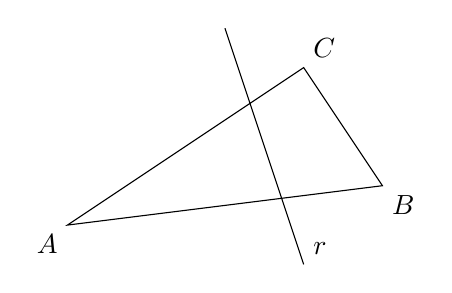
\begin{tikzpicture}
\draw (0,0) node[below left]{$A$} -- (4,.5) node[below right]{$B$} -- (3,2) node[above right]{$C$} -- cycle (3,-.5) node[above right]{$r$} -- (2,2.5);
\end{tikzpicture}
\caption{Axioma de Pasch.}
\end{figure}

M. Pasch, quién en la obra de Hilbert es creditado como el real inventor de los axiomas de orden, afirmaba que el axioma II4 había sido utilizado inconscientemente por Euclides en su obra, a pesar de ser indemostrable con su conjunto original.
\begin{mydef}[Segmento]
Definimos el segmento\index{segmento} $\overline{AB}$\nomenclature{$\overline{AB}$}{Segmento de extremos $A$ y $B$} como tal que contiene todos los puntos (de $AB$) entre $A$ y $B$ (estos últimos incluidos). Usualmente llamamos a la recta $AB$ como la \textit{prolongación}\index{prolongación!de un segmento} de $\overline{AB}$.
\end{mydef}
\begin{thm}[Primer teorema de Pasch]\index{teorema!de Pasch, primero}
Dada la situación de II4, podemos ver que la recta sólo puede estar entre $A$ y $C$ o $B$ y $C$, pero no ambas simultáneamente.
\end{thm}
\begin{proof}
Demostremos esto por contradicción. Supongamos que $r$ intersecta $\overline{AB}$ en $A'$, intersecta a $\overline{AC}$ en $B'$ y a $\overline{BC}$ en $C'$. Veamos que $A',B',C'$ deben ser distintos, por ejemplo, si $A'=B'$, entonces $A,B,C$ serían colineales. Por II3 podemos suponer que $A'-B'-C'$.

Como $r$ no intersecta a $B$ los puntos $B,A',C'$ no son colineales. La recta $AC$ intersecta a $B'$ que está entre $A'C'$, luego por axioma de Pasch, $AC$ debe pasar entre $\overline{A'B}$ o $\overline{BC'}$. Sin embargo, $A'B=AB$ y $BC'=BC$, luego los únicos puntos por los que puede pasar son $A$ o $B$, pero por II3 no se cumple ni $A'-A-B$ ni $B-C-C'$, contradicción.
\end{proof}
\begin{thm}[Segundo teorema de Pasch]\index{teorema!de Pasch, segundo}
Dados cuatro puntos colineales distintos, se pueden elegir de forma tal que $A$, $B$, $C$ y $D$ estén en orden (es decir, que $A-B-C$, $A-B-D$, $B-C-D$ y $A-C-D$).
\end{thm}
\begin{proof}
Denotaremos $l$ la recta que contiene los cuatro puntos. Consideremos primero, que se eligen tres puntos cualesquiera y se nombran tales que $A-B-C$, luego se eligen $B,C,D$ con lo que podemos obtener que $D-B-C$, $B-D-C$ o $B-C-D$ (II3).
\begin{enumerate}
\item $D-B-C$. Alternaremos las etiquetas de $A$ con $C$, de forma que tengamos que $A-B-C$ y $A-B-D$. Con ello, probaremos que $B$ no puede estar entre $C$ y $D$.

Para esa demostración comenzaremos por considerar un punto $E$ no colinear con $A,B$ (I7), y luego, un $F$ tal que $E-A-F$ (II2). Luego, veremos que $EB$ intersecta a $\overline{AC}$ y $\overline{AD}$ (en $B$) y que no puede intersectar a $\overline{AF}$ (pues si lo hiciese se daría que $E-B-F$, contradiciendo que $A\neq B$), por ende, intersecta a $\overline{FC}$ y $\overline{FD}$ (axioma de Pasch). Finalmente, por el primer teorema de Pasch, $EB$ no intersecta a $\overline{CD}$, como se quería probar.
\begin{figure}
\centering
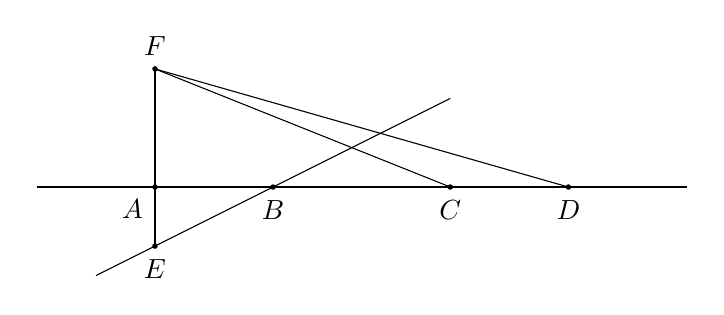
\begin{tikzpicture}[scale=.75]
	\node (0) at (-4, 0) {};
	\node[circle, fill=black, inner sep=0pt,minimum size=2,label=below left:{$A$}] (1) at (-2, 0) {};
	\node[circle, fill=black, inner sep=0pt,minimum size=2,label=below:{$B$}] (2) at (0, 0) {};
	\node[circle, fill=black, inner sep=0pt,minimum size=2,label=below:{$C$}] (3) at (3, 0) {};
	\node[circle, fill=black, inner sep=0pt,minimum size=2,label=below:{$D$}] (4) at (5, 0) {};
	\node (5) at (7, 0) {};
	\node[circle, fill=black, inner sep=0pt,minimum size=2,label=above:{$F$}] (6) at (-2, 2) {};
	\node[circle, fill=black, inner sep=0pt,minimum size=2,label=below:{$E$}] (7) at (-2, -1) {};
	\node (8) at (3, 1.5) {};
	\node (9) at (-3, -1.5) {};
	\draw (0.center) to (5.center);
	\draw (9.center) to (8.center);
	\draw (7.center) to (6.center);
	\draw (6.center) to (3.center);
	\draw (6.center) to (4.center);
\end{tikzpicture}
\end{figure}

Esto nos deja con que $B-C-D$ ó $B-D-C$. En el segundo caso alternamos las etiquetas de $D$ con $C$.
\item $B-D-C$. Alternaremos las etiquetas de $C$ con $D$, de forma que $A-B-D$ y $B-C-D$. Ahora, probaremos que $A-C-D$ y que $A-B-C$.

Sabemos que existen puntos que no pertenecen a $l$, así que llamemos $E$ a uno de ellos, y luego $F$ como un punto tal que $D-E-F$. Luego, sabemos que $FB$ intersecta a $\overline{AD}$ en $B$ y que no puede intersectar a $\overline{ED}$ (pues $D-E-F$ y la intersección de rectas es única), por ende, intersecta a $\overline{AE}$ en $G$. Ahora consideremos la recta $BG$ y su relación a los puntos $C,D,E$. Evidentemente $BG$ no intersecta a $\overline{CD}$, puesto que dos rectas sólo se intersectan en punto, que en este caso es $B$ y sabemos que $B-C-D$. $BG$ tampoco intersecta a $\overline{DE}$ por el mismo argumento, ya que $F\in BG$. Por ende, $BG$ tampoco intersecta a $\overline{CE}$. Finalmente, consideremos $BG$ con $A,C,E$: intersecta a $\overline{AE}$ en $G$, pero no a $\overline{CE}$, por ende, intersecta a $\overline{AC}$ y debe ser en $B$. Es decir, $A-B-C$.
\begin{figure}
\centering
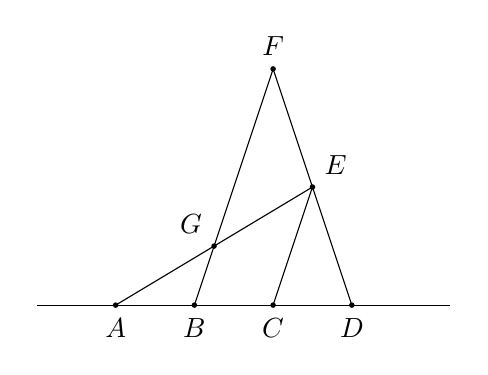
\begin{tikzpicture}
	\node (0) at (-3.25, 0) {};
	\node[circle, fill=black, inner sep=0pt, minimum size=2, label=below:{$A$}] (1) at (-2.25, 0) {};
	\node[circle, fill=black, inner sep=0pt, minimum size=2, label=below:{$B$}] (2) at (-1.25, 0) {};
	\node[circle, fill=black, inner sep=0pt, minimum size=2, label=below:{$C$}] (3) at (-0.25, 0) {};
	\node[circle, fill=black, inner sep=0pt, minimum size=2, label=below:{$D$}] (4) at (0.75, 0) {};
	\node (5) at (2, 0) {};
	\node (6) at (2, 0) {};
	\node[circle, fill=black, inner sep=0pt, minimum size=2, label=above right:{$E$}] (7) at (0.25, 1.5) {};
	\node[circle, fill=black, inner sep=0pt, minimum size=2, label=above:{$F$}] (8) at (-0.25, 3) {};
	\node[circle, fill=black, inner sep=0pt, minimum size=2, label=above left:{$G$}] (9) at (-1, 0.75) {};
	\draw (0.center) to (6.center);
	\draw (8.center) to (4.center);
	\draw (8.center) to (2.center);
	\draw (7.center) to (1.center);
	\draw (7.center) to (3.center);
\end{tikzpicture}
\end{figure}

Para la demostración restante analizaremos la relación entre $GC$ y $A,B,E$: $GC$ intersecta a $\overline{AE}$ en $G$ y no puede intersectar a $\overline{AB}$ puesto que $A-B-C$ y sólo puede intersectar a $l$ en un punto; por ende intersecta a $\overline{BG}$ en $H$. Luego, sabemos que intersecta a $\overline{BE}$ en $H$ y a $\overline{BD}$ en $C$, por lo que, por teorema de Pasch, no intersecta a $\overline{DE}$. Finalmente, intersecta  a $\overline{AE}$ en $G$, pero no a $\overline{DE}$, por lo que intersecta a $\overline{AD}$ y debe ser en $C$, es decir, $A-C-D$.
\begin{figure}
\centering
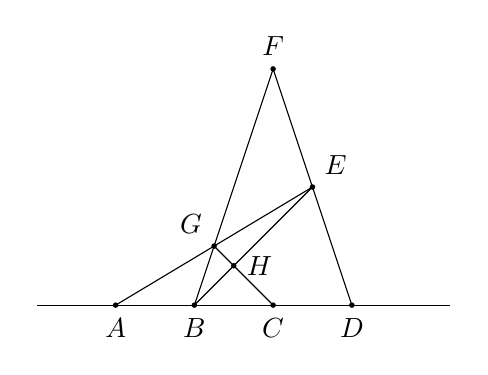
\begin{tikzpicture}
	\node (0) at (-3.25, 0) {};
	\node[circle, fill=black, inner sep=0pt, minimum size=2, label=below:{$A$}] (1) at (-2.25, 0) {};
	\node[circle, fill=black, inner sep=0pt, minimum size=2, label=below:{$B$}] (2) at (-1.25, 0) {};
	\node[circle, fill=black, inner sep=0pt, minimum size=2, label=below:{$C$}] (3) at (-0.25, 0) {};
	\node[circle, fill=black, inner sep=0pt, minimum size=2, label=below:{$D$}] (4) at (0.75, 0) {};
	\node (5) at (2, 0) {};
	\node (6) at (2, 0) {};
	\node[circle, fill=black, inner sep=0pt, minimum size=2, label=above right:{$E$}] (7) at (0.25, 1.5) {};
	\node[circle, fill=black, inner sep=0pt, minimum size=2, label=above:{$F$}] (8) at (-0.25, 3) {};
	\node[circle, fill=black, inner sep=0pt, minimum size=2, label=above left:{$G$}] (9) at (-1, 0.75) {};
	\node[circle, fill=black, inner sep=0pt, minimum size=2, label=right:{$H$}] (10) at (-0.75, 0.5) {};
	\draw (0.center) to (6.center);
	\draw (8.center) to (4.center);
	\draw (8.center) to (2.center);
	\draw (7.center) to (1.center);
	\draw (9.center) to (3.center);
	\draw (7.center) to (2.center);
\end{tikzpicture}
\end{figure}
\item Como $A-B-C$ y $B-C-D$, debemos probar que $A-B-D$ y que $A-C-D$. En particular, probaremos el primero ya que los casos son simétricos. Comenzamos por ver que debe existir $E\notin l$ (I7) y que también existe $F$ tal que $A-E-F$ (II2). Luego, sabemos que $FB$ intersecta a $\overline{AC}$ en $B$ y que no puede intersectar a $\overline{AE}$ puesto que $A-E-F$, por lo que $FB$ intersecta a $\overline{CE}$ en $G$ (II4). Asimismo, sabemos que $FB$ no puede intersectar a $\overline{CD}$ pues $B-C-D$, por lo que intersecta a $\overline{DE}$ en $H$ (II4). Finalmente $FB$ intersecta a $\overline{DE}$, pero no a $\overline{AE}$, por lo que debe intersectar a $\overline{AD}$ en $B$, osea, $A-B-D$.
\begin{figure}
\centering
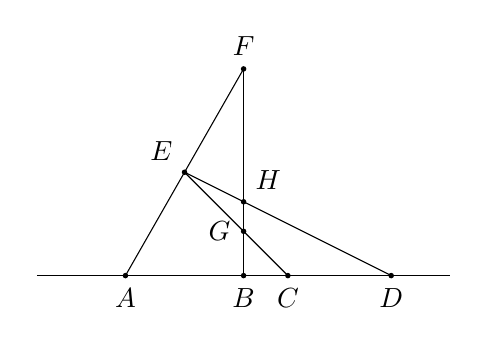
\begin{tikzpicture}[scale=.75]
	\node (0) at (-3, 0) {};
	\node[circle, fill=black, inner sep=0pt, minimum size=2, label=below:{$A$}] (1) at (-1.5, 0) {};
	\node[circle, fill=black, inner sep=0pt, minimum size=2, label=below:{$B$}] (2) at (0.5, 0) {};
	\node[circle, fill=black, inner sep=0pt, minimum size=2, label=below:{$C$}] (3) at (1.25, 0) {};
	\node[circle, fill=black, inner sep=0pt, minimum size=2, label=below:{$D$}] (4) at (3, 0) {};
	\node (5) at (4, 0) {};
	\node[circle, fill=black, inner sep=0pt, minimum size=2, label=above left:{$E$}] (6) at (-0.5, 1.75) {};
	\node[circle, fill=black, inner sep=0pt, minimum size=2, label=above:{$F$}] (7) at (0.5, 3.5) {};
	\node[circle, fill=black, inner sep=0pt, minimum size=2, label=left:{$G$}] (8) at (0.5, 0.75) {};
	\node[circle, fill=black, inner sep=0pt, minimum size=2, label=above right:{$H$}] (9) at (0.5, 1.25) {};
	\draw (0.center) to (5.center);
	\draw (1.center) to (7.center);
	\draw (6.center) to (3.center);
	\draw (6.center) to (4.center);
	\draw (2.center) to (7.center);
\end{tikzpicture}
\end{figure}
\end{enumerate}
Nótese que por las demostraciones dadas en 2, del primer caso se concluye inmediatamente todos los ordenes requeridos.
\end{proof}
\begin{thm}\label{thm:intermediate-point}
Entre dos puntos siempre existe un tercero.
\end{thm}
\begin{proof}
Llamemos $A,B$ dos puntos sobre un plano, por I7 existe un punto fuera de la recta $X$, por II2 existe $C$ tal que $A-X-C$, asimismo, existe $Y$ tal que $B-C-Y$, luego $A,B,C$ son puntos no colineales e $YX$ una recta que pasa por $\overline{AC}$, luego, pasa por $\overline{BC}$ o $\overline{AB}$ (además es claro que $XY$ no pasa por $A,B,C$, de lo contrario, son colineales). Pero como $B,C,Y$ son colineales, $X$ tendría que estar en la misma recta para satisfacerlo y es evidente que no es así (de lo contrario $XY=BC$ y se llega a que $A,B,C$ son colineales), finalmente, $XY$ corta a $\overline{AB}$ y dicho punto está entre ambos (y no es ni $A$ ni $B$).
\end{proof}
\begin{figure}[!ht]
\centering
\begin{tikzpicture}[scale=.75]
\draw (0,0) node[below left]{$A$} -- (5,0) node[below right]{$B$};
\draw (0,0) -- (1.44,2.2) node[above left]{$X$} -- (2.61,3.98) node[above right]{$C$} -- (5,0) (2.61,3.98) -- (2,5) node[above]{$Y$} -- (1,0);
\end{tikzpicture}
\caption{Teorema~\ref{thm:intermediate-point}.}
\end{figure}

\begin{cor}
Todo segmento posee infinitos puntos (exceptuando los de tipo $\overline{AA}$).
\end{cor}
\begin{thm}
Sea $a$ una recta en un plano $\alpha$. Entonces la relación sobre $\alpha\setminus a$\footnote{$a\setminus b$ se interpreta como los elementos de $a$ que no están en $b$.}
$$P\sim_a Q\iff P=Q\vee\overline{PQ}\text{ no intersecta a }a$$
\nomenclature{$\iff$}{Si y sólo si\nomnorefpage}
\nomenclature{syss}{Si y sólo si\nomnorefpage}
\nomenclature{$\vee$}{Disjunción (``o'' lógico)\nomnorefpage}
es de equivalencia\index{relación!de equivalencia}\footnote{Es decir, posee reflexividad\index{reflexividad!de una relación} ($P\sim_a P$), simetría\index{simetría!de una relación} ($P\sim_a Q\iff Q\sim_a P$) y transitividad\index{transitividad} ($P\sim_a Q$ y $Q\sim_a R\implies P\sim_a R$).}
\nomenclature{$\implies$}{Entonces\nomnorefpage}
y determina dos clases de equivalencia.
\end{thm}
\begin{proof}
Es trivial la reflexividad y simetría de la relación. Vamos a probar la transitividad. Supongamos por contradicción que $\overline{PR}$ intersecta a $a$, sabemos que como $\sim_a$ no incluye puntos en $a$, los puntos $P,Q,R$ no están contenidos en $a$. Si los puntos son no colineales por axioma de Pasch, $a$ debería intersectar a $\overline{PQ}$ o $\overline{QR}$. Si los puntos son colineales, entonces como $a$ intersecta $\overline{PR}$ debe intersectar a $\overline{PQ}$ o a $\overline{QR}$ (pues la unión de ambos segmentos es $\overline{PR}$), lo cual es absurdo.

Ahora probemos que hay sólo dos clases de equivalencia: Tómese $A\in\alpha\setminus a$\nomenclature{$\in$}{Pertenece al conjunto\nomnorefpage}\nomenclature{$\setminus$}{Resta (de conjuntos)\nomnorefpage} y $X\in a$, por II2 existe $B$ tal que $A-X-B$, luego $A\not\sim_a B$, lo cual significa que hay al menos dos clases de equivalencia. Probaremos que dado cualquier otro $C\in\alpha\setminus a$ está en la clase de $A$ o en la de $B$. Supongamos que no son colineares, luego por primer teorema de Pasch, $a$ intersecta a $\overline{AC}$ o a $\overline{BC}$, pero no los dos simultáneamente, es decir, $C$ está o en la clase de $A$ o en la de $B$, pero no en ambas (como se quería). Si $A,B,C$ son colineares, por I7 podemos tomar un $Y$ tal que no pertenece a $AB$ y está sobre $a$; luego por II2 existe $D$ tal que $Y-C-D$, es decir, $C\sim_a D$, como $D$ no está en $AB$ podemos aplicar el razonamiento anterior y la transitividad para ver que $C$ está en la clase de $A$ o de $B$.
\end{proof}
Usualmente estas dos clases usualmente se llaman \textit{semiplanos}\index{semiplano}, y el lector debe interpretar la idea de \textit{dos clases de equivalencia} como decir ``toda recta $a$ en un plano $\alpha$ lo corta en dos semiplanos''.
\begin{thm}
Sea $A$ un punto de una recta $a$. Definimos la relación en $a\setminus\{A\}$
$$P\sim_A Q\iff P=Q\vee A\notin\overline{PQ}$$
es de equivalencia y determina exactamente dos clases de equivalencia.
\end{thm}
\begin{proof}
Tomemos un $X$ externo a $a$, luego definamos $b=AX$; además, como $a$ y $b$ son rectas distintas que se intersectan en $A$ definen un plano $\alpha$. Luego se comprueba para puntos de $a\setminus\{A\}$ que
$$P\sim_A Q\iff P\sim_b Q,$$
con lo que se comprueba que $\sim_A$ es relación de equivalencia y posee al menos dos clases. Para comprobarlo basta considerar un par $P,Q$ tal que $P-A-Q$.
\end{proof}
Nuevamente, estas dos clases deben interpretarse como las llamadas \textit{semirrectas}\index{semirrecta} (a veces también llamados \textit{rayos}\index{rayo}).
\begin{mydef}[Rayo o semirrecta]
Se le dice rayo o semirrecta a $\overrightarrow{AB}$\nomenclature{$\overrightarrow{AB}$}{Rayo de origen $A$ que pasa por $B$} como la clase de equivalencia que contiene a $B$ a partir de la relación $P\sim_A Q$ sobre la recta $AB$ (más el mismo punto $A$), a $A$ le decimos el \textit{origen}\index{origen!de un rayo} de $\overrightarrow{AB}$. A la recta $AB$ le llamamos la \textit{prolongación}\index{prolongación!de una semirrecta} de $\overrightarrow{AB}$, y si $C-A-B$ con $C\neq A$, vemos que $\overrightarrow{AC}$ es la menor semirrecta tal que $CB=\overrightarrow{AB}\cup\overrightarrow{AC}$\nomenclature{$\cup$}{Unión (de conjuntos)\nomnorefpage}, a ella le llamamos \textit{semirrecta complementaria}\index{semirrecta!complementaria}.
\end{mydef}
\begin{mydef}[Semiplano]
Sea $\alpha$ un plano y $a$ una recta contenida en él\footnote{Con ``contenido'' nos referimos a que $a \subset\alpha$\nomenclature{$\subset,\subseteq$}{Subconjunto propio e impropio, resp\nomnorefpage}.}, luego se define un \textit{semiplano} con \textit{frontera}\index{frontera!de un semiplano} $a$ como una de las clases de equivalencias de la relación $P\sim_a Q$ sobre $a\setminus\alpha$, unidos a la misma frontera. Dado un semiplano, el plano original (que es único por I3) se le dice su \textit{prolongación}\index{prolongación!de un semiplano}. Al otro semiplano se le llama \textit{complementario}\index{semiplano!complementario}.
\end{mydef}
\begin{thm}
Dado $A-B-C$ con $A\neq B\neq C$, entonces
$$\overline{AB}\cap\overline{BC}=\{B\},\quad\overline{AC}=\overline{AB}\cup\overline{BC}.$$
\nomenclature{$\cap$}{Intersección (de conjuntos)\nomnorefpage}
\end{thm}
\begin{proof}
Supongamos que $P\neq B$, probaremos por contradicción que $P$ no puede estar en $\overline{AB}$ y $\overline{BC}$. Si estuviera satisface que $P\sim_B A$ y $P\sim_B C$, por transitividad, $A\sim_B C$ lo cual es contradictorio.

Vamos a demostrar que si $X\in\overline{AB}$ entonces $X\in\overline{AC}$. Si $X=A$ o $X=B$ es trivial. En caso contrario, escogiremos un $Y$ externo a $AC$, y un $Z$ tal que $A-Y-Z$. Veamos que $XY$ intersecta a $AC$ en $X$ en $\overline{AB}$, por el teorema anterior, no pasa por $\overline{BC}$, luego, si pasara por $\overline{ZC}$ tendría que pasar por $\overline{ZB}$ (por axioma de Pasch) lo cual no ocurre por el teorema de Pasch aplicado a $A,B,Z$. Finalmente por axioma de Pasch aplicado a $ACZ$ sabemos que $XY$ intersecta a $\overline{AC}$, específicamente en $X$, es decir, $X\in\overline{AC}$.
\begin{figure}[!ht]
\centering
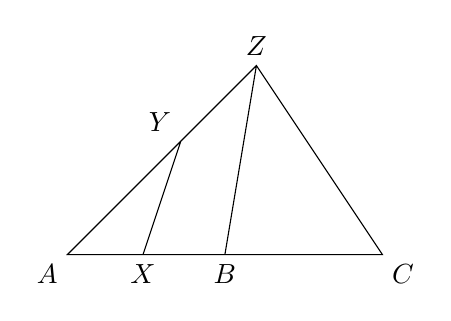
\begin{tikzpicture}[scale=.8]
\draw (0,0) node[below left]{$A$} -- (2.5,0) node[below]{$B$} -- (5,0) node[below right]{$C$} -- (3,3) node[above]{$Z$} -- cycle (2.5,0) -- (3,3) (1.8, 1.8) node[above left]{$Y$} -- (1.2, 0) node[below]{$X$};
\end{tikzpicture}
\end{figure}

Como $A-X-C$ es equivalente a $C-X-A$, lo mismo se aplica a $X\in\overline{BC}$ implica $X\in\overline{AC}$. Finalmente como $XY$ pasa por $\overline{AZ}$, por teorema de Pasch, pasa por $\overline{AB}$ o $\overline{BZ}$, en cuyo último caso, por axioma de Pasch, pasa por $\overline{BC}$.
\end{proof}
\begin{mydef}
A un conjunto $C$ de puntos se le dice \textit{convexo}\index{convexo} syss para todo $P,Q\in C$ se cumple que si $P-X-Q$ entonces $X\in C$. De lo contrario se le dice \textit{cóncavo}\index{concavo@cóncavo}.
\end{mydef}
Veamos que las rectas, planos, segmentos y semirrectas son trivialmente convexos. Queda como ejercicio para el lector probar que los semiplanos también lo son.

\subsection*{Axiomas de congruencia}
En lo sucesivo, se debe interpretar que la congruencia es algo así como la cualidad de ser iguales en medida y forma.
\begin{axiom}[IV, 1]
Todas las congruencias de figuras (denotadas por el signo $\equiv$) \nomenclature{$\equiv$}{Congruentes} son relaciones de equivalencia.
\end{axiom}
\begin{axiom}[IV, 2]
Dado un par de puntos distintos $A,\,B$ y una semirrecta $s$ de origen $C$, existe un único $D\in s$ tal que $\overline{AB}\equiv\overline{CD}$.
\end{axiom}
\begin{axiom}[IV, 3]
Sean $A-B-C$ distintos y colineales; y sean $A'-B'-C$ distintos y colineales también, tales que
$$\overline{AB}=\overline{A'B'},\quad\overline{BC}=\overline{B'C'},$$
entonces $\overline{AC}=\overline{A'C'}$.
\end{axiom}
\begin{mydef}[Ángulo]
Sean $h,k$ dos rayos de mismo origen $O$, cuyas prolongaciones son $r_1, r_2$ respectivamente sobre un plano $\alpha$. Definimos el \textit{ángulo}\index{angulo@ángulo} como un conjunto denotado $\angle(h,k)$
\nomenclature{$\angle$}{Ángulo}
tal que corresponde a la intersección del semiplano de frontera $r_1$ que contiene a $k$ y el semiplano de frontera $r_2$ que contiene a $h$. Usualmente a $h,k$ le llamamos \textit{lados}\index{lado!de un ángulo} del ángulo, mientras que a $O$ le llamamos el \textit{vértice}\index{vertice@vértice!de un ángulo}.
\end{mydef}
Finalmente, sean $h',k'$ los complementos de los rayos $h,k$ respectivamente. A $\angle(h',k)$ y $\angle(h,k')$ les llaman \textit{ángulos adyacentes}\index{angulo@ángulo!adyacente}, mientras que a $\angle(h',k')$ le llamamos \textit{ángulo opuesto por el vértice}\index{angulo@ángulo!opuesto por el vértice}.
\begin{figure}[!ht]
\centering
\begin{tikzpicture}[scale=1.25]
\begin{scope}
\clip (0,0) rectangle (5,3);
\draw (5,4) -- (0,-1) (7,2) -- (-1,1);
\filldraw[body] (5,4) -- node[sloped, above]{$h$} (2.4, 1.4) node[below right]{$O$} -- node[sloped, below]{$k$} (7,2);
\end{scope}
\draw (0,0) -- (5,0) -- (5,3) node[above right]{$\alpha$} -- (0,3) -- cycle (4,2.2) node {$\angle(h,k)$} (1.4,2.2) node {Ángulo adyacente} (3.6, .6) node {Ángulo adyacente} (.8,.8) node {Opuesto};
\end{tikzpicture}
\caption{Ángulos.}
\end{figure}

Además, para simplificar notación, sean $A,O,B$ puntos no colineales, definimos $\angle AOB\equiv\angle(\overrightarrow{OA},\overrightarrow{OB})$.
\begin{thm}[Teorema de las barras cruzadas]\index{teorema!de las barras cruzadas}
Sea $\angle AOB$ contenido en $\alpha$, una semirrecta de origen $O$ está contenida en $\angle AOB$ syss intersecta a $\overline{AB}$.
\end{thm}
\begin{proof}
$\implies$. Por II2 existe $C$ tal que $A-O-C$, luego $A,B,C$ son no colineales y la prolongación de $s$ corta a $\overline{AC}$ en $O$, por axioma de Pasch, corta a $\overline{BC}$ o $\overline{AB}$. Mas, no puede intersectar a $\overline{BC}$ pues este pertenece al ángulo $\angle BOC$ que es adyacente a $\angle AOB$, esto debido, a que su semirrecta complementaria, como pasa por $O$, cruza ambos lados quedando así en el ángulo opuesto. Por ende, cruza a $\overline{AB}$ y debe ser $s$ quién lo haga pues su complemento está en el ángulo opuesto.
\begin{figure}
\centering
\begin{tikzpicture}[scale=.8]
	\node[circle, fill=black, inner sep=0pt, minimum size=2, label=below:{$O$}] (0) at (0, 0) {};
	\node[circle, fill=black, inner sep=0pt, minimum size=2, label=below:{$A$}] (1) at (3, 0) {};
	\node[circle, fill=black, inner sep=0pt, minimum size=2, label=below left:{$C$}] (2) at (-3, 0) {};
	\node[circle, fill=black, inner sep=0pt, minimum size=2, label=above left:{$B$}] (3) at (3, 3) {};
	\node[label=right:{$s$}] (4) at (4, 2) {};
	\node (5) at (-2.5, -1.25) {};
	\node (6) at (3, 1.5) {};
	\node (7) at (4, 4) {};
	\node (8) at (4, 0) {};
	\draw (0.center) to (4.center);
	\draw[dashed] (5.center) to (0.center);
	\draw (0.center) to (1.center);
	\draw[dashed] (0.center) to (2.center);
	\draw[dashed] (1.center) to (3.center);
	\draw[dashed] (2.center) to (3.center);
	\draw (0.center) to (3.center);
	\draw (3.center) to (7.center);
	\draw (1.center) to (8.center);
\end{tikzpicture}
\end{figure}

$\Longleftarrow$. Supongamos que $s$ intersecta a $\overline{AB}$ en $C$ y sea $D\in s$ distinto de $O$, entonces la prolongación de $\overline{CD}$ corresponde a la prolongación de $s$. Como $O\notin\overline{CD}$ entonces está en los mismos semiplanos que los lados del ángulo, por ende, $\overline{CD}\subset\angle AOB$ y, en general, $s\in\angle AOB$ (puesto que todo punto $C\in s$ está en el ángulo).
\end{proof}
\begin{axiom}[IV, 4]
Sea $\theta_1$ un ángulo, y $s$ una semirrecta de prolongación $r$ y $\alpha$ un semiplano de frontera $r$ que contiene a $s$; existe un único ángulo $\theta_2$ en $\alpha$ tal que uno de sus lados sea $s$ que satisface $\theta_1\equiv\theta_2$.
\end{axiom}
\begin{mydef}[Triángulo]
Sean $A,B,C$ no colineales, entonces se define el \textit{triángulo}\index{triangulo@triángulo} denotado $\triangle ABC$\nomenclature{$\triangle ABC$}{Triángulo de vértices $A$, $B$ y $C$}
como la intersección entre $\angle ABC$, $\angle BCA$ y $\angle CAB$.
\end{mydef}
\begin{figure}[!ht]
\centering
\begin{tikzpicture}
\filldraw[body] (1.2,.6) node[below left]{$A$} -- (4,1) node[below right]{$B$} -- (2.4,2.2) node[above]{$C$} -- cycle;
\draw (0,0) -- (5,0) -- ++(0,3) node[below left]{$\alpha$} -- (0,3) -- cycle;
\end{tikzpicture}
\caption{Triángulo.%\footnote{El interior está pintado para dar a entender que todos esos puntos pertenecen al triángulo, no obstante, para evitar colapsar la pantalla, en lo sucesivo sólo dibujaremos la frontera del mismo (aun que aún no definimos dicho concepto con rigurosidad).}
}
\end{figure}

En lo siguiente diremos que un par de triángulos $\triangle ABC$ y $\triangle A'B'C'$ son congruentes cuando sus lados y ángulos \textbf{respectivos} lo son:
$$\begin{array}{rclrclrcl}
\overline{AB}&\equiv&\overline{A'B'} &\overline{BC}&\equiv&\overline{B'C'} &\overline{CA}&\equiv&\overline{C'A'}\\
\angle A&\equiv&\angle A' &\angle B&\equiv&\angle B' &\angle C&\equiv&\angle C' 
\end{array}$$
\begin{axiom}[IV, 5]
Sea $\triangle ABC$ y $A',\,B'$ un par de puntos tales que $\overline{AB}\equiv\overline{A'B'}$, entonces dado un semiplano $\alpha$ de frontera $A'B'$, existe un único $C'\in\alpha$ tal que $\triangle ABC\equiv\triangle A'B'C'$.
\end{axiom}

\section{Segmentos y triángulos}
\begin{thm}
Dados dos segmentos $\overline{AB},\,\overline{CD}$ existe $\overline{PQ}$ tal que existe $R\in\overline{PQ}$ tal que $\overline{PR}\equiv\overline{AB}$ y $\overline{RQ}\equiv\overline{CD}$.
\end{thm}
\begin{proof}
Se desprende inmediatamente del axioma IV 2; debido a que primero se elige $P$ y otro punto cualquiera para construir una recta $r$ y elegir de ella una semirrecta. Con ella, construimos $R$ para que satisfaga el enunciado. Luego, construimos la semirrecta de $r$ de origen $R$ que no contiene a $P$ para que apliquemos el axioma IV 2 y construyamos $Q$.
\end{proof}
\begin{mydef}
En condiciones del teorema anterior, escribiremos
$$\overline{PQ}\equiv\overline{AB}+\overline{CD}$$
a lo que referiremos como \textit{suma de segmentos}\index{suma!de segmentos}.
\end{mydef}
\begin{thm}
$\overline{PQ}\equiv a+b$ syss existe un único $R\in\overline{PQ}$ tal que $\overline{PR}\equiv a$ y $\overline{RQ}\equiv b$.
\end{thm}
\begin{thm}
Sean $a,b,c$ segmentos tales que $a+b\equiv a+c$, entonces, $b=c$.
\end{thm}
\begin{proof}
Sea $a+b\equiv\overline{PQ}$, entonces existe $R\in\overline{PQ}$ tal que $a\equiv\overline{PR}$ y $b\equiv\overline{RQ}$. Por el mismo argumento, existe $R'\in\overline{PQ}$ tal que $a\equiv\overline{PR'}$ y $c\equiv\overline{R'Q}$, pero por unicidad de dicho punto tenemos que $R=R'$ con lo que se demuestra el resultado.
\end{proof}
\begin{mydef}
Sean $a,b$ segmentos cualesquiera, denotaremos que $a\lt b$ \nomenclature{$a\lt b$}{Segmento $a$ menor que $b$.} (léase ``$a$ menor que $b$'') syss existe un segmento $c$ tal que $b\equiv a+c$. También, escribiremos $a\leq b$ syss $a\lt b$ o $a\equiv b$.
\end{mydef}

\subsection*{Criterios de congruencia entre triángulos}
En lo sucesivo presentaremos tres congruencias que nos serán de vital importancia. Cabe destacar que debido a la extensión de sus nombres, al aplicarlos lo haremos mediante las siglas de sus nombres. Asimismo, conservaremos el hábito de llamar a los ángulos de un triángulo por el punto de origen del mismo, excepto cuando sea absolutamente necesario.
\begin{lem}
Dados $\angle POA\equiv\angle POB$ contenidos en el mismo semiplano de frontera $PO$, entonces, $O,A,B$ son colineales y pertenecen a la misma semirrecta de origen en $O$.
\end{lem}
\begin{proof}
Por IV4 son el mismo ángulo. Luego, sabemos que uno de los lados es igual ($\overrightarrow{OP}$), luego, el otro también debe serlo $\overrightarrow{OA}=\overrightarrow{OB}$, en particular, nuestro resultado.
\end{proof}
\begin{thm}[Criterio lado-ángulo-lado]\index{criterio!lado-ángulo-lado}
Sean $\triangle ABC,\,\triangle A'B'C'$ tales que
$$\overline{AB}\equiv\overline{A'B'},\;\angle B\equiv\angle B',\;\overline{BC}\equiv\overline{B'C'},$$
entonces, $\triangle ABC\equiv\triangle A'B'C'$.
\end{thm}
\begin{proof}
Consideremos el $\triangle ABC$, el plano $\alpha=A'B'C'$ y el segmento $\overline{A'B'}$, entonces existe un único punto $P$ tal que $\triangle A'B'P\subset\alpha$ es congruente a $\triangle ABC$ (IV5). Como la congruencia es relación de equivalencia $\overline{B'C'}\equiv\overline{B'P}$ y $\angle A'B'C'\equiv\angle A'B'P$ (IV1), por el lema anterior, $B',C',P$ pertenecen a la misma semirrecta de origen $B'$, por IV2, tenemos que la unicidad del punto $P$, es decir, $C'=P$.
\end{proof}
\begin{thm}[Criterio ángulo-lado-ángulo]\index{criterio!ángulo-lado-ángulo}
Sean $\triangle ABC,\,\triangle A'B'C'$ tales que
$$\angle A\equiv\angle A',\;\overline{AB}\equiv\overline{A'B'},\;\angle B\equiv\angle B'$$
entonces, $\triangle ABC\equiv\triangle A'B'C'$.
\end{thm}
\begin{proof}
Sea $P$ en el semiplano de frontera $A'B'$ que contiene a $C'$ tal que $\triangle ABC\equiv\triangle A'B'P$. Por IV4, $\angle C'A'B'=\angle PA'B'$ y $\angle A'B'C'=\angle A'B'P$, por ende, $\overrightarrow{A'C'}=\overrightarrow{A'P}$ y $\overrightarrow{B'C'}=\overrightarrow{B'P}$. Finalmente, por unicidad de la intersección, $C'=P$.
\end{proof}
\begin{thm}\label{thm:angle-sum-1}
Sean $s_1,s_2,s_3$ semirrectas de origen $O$ que pueden ubicarse en un mismo semiplano cuya frontera incluya a $O$; $s_1^\prime, s_2^\prime, s_3^\prime$ semirrectas de origen $O'$ en las mismas condiciones. Si $s_2\in\angle(s_1,s_3)$, $\angle(s_1,s_2)\equiv\angle(s_1^\prime,s_2^\prime)$ y $\angle(s_1,s_3)\equiv\angle(s_1^\prime,s_3^\prime)$, entonces, $s_2^\prime\in\angle(s_1^\prime,s_3^\prime)$ y $\angle(s_2,s_3)\equiv\angle(s_2^\prime,s_3^\prime)$.
\end{thm}
\begin{proof}
Escójase $A\in s_1$ y $B\in s_3$ cualesquiera (excepto $O$ mismo), por teorema de las barras cruzadas sabemos que $s_2$ corta a $\overline{AB}$ en $C$. Luego, sean $A'\in s_1^\prime$ y $B'\in s_3^\prime$ tales que $\overline{OA}\equiv\overline{O'A'}$ y $\overline{OB}\equiv\overline{O'B'}$ (IV). Por LAL, $\triangle AOB\equiv\triangle A'O'B'$, por lo cual, $\angle OAB\equiv\angle O'A'B'$. Digamos que sea $C'$ la intersección entre la prolongación de $s_2^\prime$ y $A'B'$, entonces, como $C'\in\overrightarrow{A'B'}$ se tiene que $\angle O'A'B'=\angle O'A'C'$, con lo que, por ALA $\triangle AOC\equiv\triangle A'O'C'$, de lo que se concluye que $\overline{AC}\equiv\overline{A'C'}$ que es menor a $\overline{A'B'}$, por lo que, $s_2^\prime$ intersecta a $\overline{A'B'}$.

Por cancelación de la suma de segmentos llegamos a probar que $\overline{BC}\equiv\overline{B'C'}$, y análogo a la prueba de la equivalencia de ángulos previamente dada vemos que $\angle OBC\equiv\angle O'B'C'$, lo que, por LAL, nos permite ver que $\triangle OBC\equiv\triangle O'B'C'$; con lo que concluimos que $\angle(s_2,s_3)=\angle COB\equiv\angle C'O'B'=\angle(s_2^\prime,s_3^\prime)$ como se quería probar.
\end{proof}
\begin{thm}\label{thm:angle-sum-2}
Sean $s_1,s_2,s_3$ semirrectas de origen $O$ en el mismo contexto que el teorema anterior. Si $\angle(s_1,s_2)\equiv\angle(s_1^\prime, s_2^\prime)$ y $\angle(s_2,s_3)\equiv\angle(s_2^\prime,s_3^\prime)$, entonces $\angle(s_1,s_3)\equiv\angle(s_1^\prime, s_3^\prime)$.
\end{thm}
\begin{proof}
Dada la prolongación de $s_1^\prime$ y el plano que contiene a $s_2^\prime$, construimos $s_3^{\prime\prime}$ como aquella semirrecta tal que $\angle(s_1,s_3)\equiv\angle(s_1^\prime,s_3^{\prime\prime})$. Luego, como $
\angle(s_1,s_2)\equiv\angle(s_1^\prime,s_2^\prime)$, por construcción, por el teorema anterior se comprueba que $\angle(s_2^\prime,s_3^\prime)\equiv\angle(s_2,s_3)\equiv\angle(s_2^\prime,s_3^{\prime\prime})$. Y por unicidad de la semirrecta, $s_3^\prime=s_3^{\prime\prime}$.
\end{proof}
\begin{mydef}
En lo sucesivo, diremos que un triángulo es \textit{equilátero}\footnote{lt. \textit{aequus}: iguales, \textit{latus, teris}: lados, costados.}\index{triangulo@triángulo!equilátero} syss todos sus lados son congruentes entre sí; diremos que es \textit{isósceles}\footnote{gr. $\acute{\iota}\sigma o\varsigma$: iguales, $\sigma\kappa\acute{\varepsilon}\lambda o\varsigma$: piernas.}\index{isosceles@isósceles} syss dos de sus lados son congruentes entre sí (en cuyo caso, llamaremos \textit{base} al lado restante) o diremos que es \textit{escaleno} si todos sus lados no son congruentes dos a dos.
\end{mydef}
\begin{thm}[Criterio de los triángulos isósceles]
Un triángulo $\triangle ABC$ es isósceles syss posee dos ángulos congruentes entre sí.
\end{thm}
\begin{proof}
$\implies$. Sin perdida de generalidad asumimos que $\overline{AC}\equiv\overline{BC}$, con lo que aplicando el criterio LAL demostramos que $\triangle ACB\equiv\triangle BCA$, por ende, $\angle A\equiv\angle B$.

$\Longleftarrow$. Sin perdida de generalidad asumimos que $\angle A\equiv\angle B$, con lo que aplicando el criterio ALA demostramos que $\triangle ACB\equiv\triangle BCA$, por ende, $\overline{AC}\equiv\overline{BC}$.
\end{proof}
Cabe notar que podemos aplicar el mismo argumento para notar que un triángulo es equilátero syss sus tres ángulos son congruentes entre sí.

Cabe destacar una especie de convenio en diagramas geométricos en el que se marcan con $n$ palos ciertos segmentos y ángulos, de forma que todos los segmentos y ángulos en la figura que tienen el mismo número de palos son congruentes entre sí. En ciertos casos, el ángulo tendrá una marca, en otros se dibujaran las líneas las veces necesarias para indicar que son congruentes (como se muestra en la figura adjunta). Cabe notar que esta no es una técnica para formalizar las demostraciones ni nada, simplemente un truco para llevar un inventario de las relaciones conocidas.
\begin{figure}
\centering
\begin{tikzpicture}
	\node (0) at (2, 0) {};
	\node (1) at (0, 0) {};
	\node (2) at (2, 1) {};
	\node (3) at (2.75, 0) {};
	\node (4) at (4.75, 1) {};
	\node (5) at (2.75, 1) {};
	\draw (0.center) to node[sloped]{$\shortmid$} (1.center) to node[sloped]{$\shortparallel$} (2.center);
	\draw (3.center) to node[sloped]{$\shortparallel$} (4.center) to node[sloped]{$\shortmid$} (5.center);
	\draw (.75,0) arc (0:{atan(1/2)}:.75);
	\draw ($(4.center)+(-.75,0)$) arc (-180:{-180+atan(1/2)}:.75);
\end{tikzpicture}
\caption{}
\end{figure}
\begin{thm}[Criterio lado-lado-lado]\index{criterio!lado-lado-lado}
Sean $\triangle ABC,\,\triangle A'B'C'$ tales que
$$\overline{AB}\equiv\overline{A'B'},\;\overline{BC}\equiv\overline{B'C'},\;\overline{CA}\equiv\overline{C'A'},$$
entonces, $\triangle ABC\equiv\triangle A'B'C'$.
\end{thm}
\begin{proof}
Veamos que dado $\triangle A'B'C'$, el semiplano complementario al de frontera $AB$ que contiene a $C$ y el segmento $\overline{AB}$ existe $C''$ tal que $\triangle A'B'C'\equiv\triangle ABC''$ (IV5).
\begin{figure}
\centering
\begin{tikzpicture}[scale=.75]
	\node[label=left:{$A$}] (0) at (-1.25, 0) {};
	\node[label=right:{$B$}] (1) at (2, 0) {};
	\node[label=above:{$C$}] (2) at (0, 3) {};
	\node[label=below:{$C''$}] (3) at (0, -3) {};
	\draw (2.center) to node[sloped]{$\shortmid$} (0.center) to node[sloped]{$\shortmid$} (3.center) to node[sloped]{$\shortparallel$} (1.center) to node[sloped]{$\shortparallel$} (2.center);
	\draw (0.center) to (1.center) (2.center) to (3.center);
	\draw ($(2.center)+({-90-atan(1.25/3)}:.5)$) arc ({-90-atan(1.25/3)}:{atan(2/3)-90}:.5) ($(2.center)+(-90:.6)$) arc (-90:{atan(2/3)-90}:.6);
	\draw ($(3.center)+({90+atan(1.25/3)}:.5)$) arc ({90+atan(1.25/3)}:{atan(3/2)}:.5) ($(3.center)+(90:.6)$) arc (90:{atan(3/2)}:.6);
\end{tikzpicture}
\end{figure}

Nótese que por teoremas~\ref{thm:angle-sum-1} y \ref{thm:angle-sum-2}, los triángulos $\triangle ACC''$ y $\triangle BCC''$ son isósceles de base $\overline{CC''}$, por lo cual, $\angle ACC''\equiv AC''C$ y $\angle C''CB\equiv\angle CC''B$, con lo que, vemos que $\angle ACB\equiv\angle AC''B\equiv A'C'B'$, por lo que, por criterio LAL queda demostrado.
\end{proof}

\section{Ángulos}
\begin{thm}
Sean $\theta,\,\theta'$ ángulos congruentes entre sí, entonces, sus ángulos adyacentes son también congruentes.
\end{thm}
\begin{proof}
Primero consideremos las semirrectas $s_1,s_2$ que forman a $\theta$: digamos que se intersectan en $O$ y que $A\in s_1$ como $B\in s_2$ (ambos distintos de $O$). Luego, sean las semirrectas $s_1^\prime,s_2^\prime$ las que forman a $\theta'$, $O'$ es su intersección y se definen $A'\in s_1^\prime,B'\in s_2^\prime$ tales que $\overline{OA}\equiv\overline{O'A'},\overline{OB}\equiv\overline{O'B'}$. Sea $C$ tal que $C-O-A$ y se define $C'$ analogamente. Lo que queremos ver es que $\angle BOC\equiv\angle B'O'C'$.
\begin{figure}
\centering
\begin{tikzpicture}
	\node[label=below:{$O$}] (0) at (0, 0) {};
	\node[label=below right:{$A$}] (1) at (2, 0) {};
	\node[label=above:{$B$}] (2) at (1, 2) {};
	\node[label=below left:{$C$}] (3) at (-2, 0) {};
	\node[label=below left:{$C'$}] (4) at (4, 0) {};
	\node[label=below:{$O'$}] (5) at (6, 0) {};
	\node[label=below right:{$A'$}] (6) at (8, 0) {};
	\node[label=above:{$B'$}] (7) at (7, 2) {};
	\draw (3.center) to node[sloped]{$\shortmid\shortparallel$} (0.center) to node[sloped]{$\shortmid$} (1.center);
	\draw (0.center) to node[sloped]{$\shortparallel$} (2.center);
	\draw (1.center) to (2.center) to (3.center);
	\draw (4.center) to node[sloped]{$\shortmid\shortparallel$} (5.center) to node[sloped]{$\shortmid$} (6.center);
	\draw (5.center) to node[sloped]{$\shortparallel$} (7.center);
	\draw (6.center) to (7.center) to (4.center);
	\draw (.75,0) arc (0:{atan(2)}:.75) ($(5.center)+(.75,0)$) arc (0:{atan(2)}:.75);
\end{tikzpicture}
\end{figure}

La información nos permite ver que $\triangle AOB\equiv\triangle A'O'B'$ por LAL, con lo que $\overline{AB}\equiv\overline{A'B'}$ y $\angle B\equiv\angle B'$. Por suma de segmentos $\overline{AC}\equiv\overline{A'C'}$, con lo que, $\triangle BAC\equiv\triangle B'A'C'$ por LAL, de lo que concluimos que $\overline{BC}\equiv\overline{B'C'}$. Finalmente $\triangle BOC\equiv\triangle B'O'C'$ por LLL, lo que comprueba el teorema.
\end{proof}
\begin{cor}
Los ángulos opuestos por el vértice son congruentes.
\end{cor}
\begin{mydef}[Ángulos complementarios]\index{angulo@ángulo!complementario}
Decimos que dos ángulos $\theta,\phi$ son complementarios syss uno es congruente a uno (y, por lo tanto, a ambos) de los ángulos adyacentes del otro.
\end{mydef}
\begin{mydef}
A los semiplanos le llamaremos \textit{ángulos llanos}\index{angulo@ángulo!llano} y los trataremos como si fuesen, efectivamente, ángulos. Así mismo, llamaremos \textit{ángulos nulos}\index{angulo@ángulo!nulo} a aquellos formados por una única semirrecta. De esta forma, admitimos que todos los llanos (resp. nulos) son congruentes entre sí, que los nulos y llanos son ``complementarios'' por definición, que los nulos son menores que cualquier otro ángulo, y que los llanos son mayores que cualquier otro.
\end{mydef}
\begin{thm}
Dado cualquier par distinto de puntos $A,\,B$ existe un único $M$ (que llamaremos punto medio) colineal a ambos tal que $A-M-B$ y $\overline{AM}\equiv\overline{MB}$.
\end{thm}
\begin{proof}
Sea $C$ un punto cualquiera externo a $AB$, existe $D$ en el semiplano complementario tal que $\triangle ABC\equiv\triangle BAD$. Por definición del semiplano, $\overline{CD}$ intersecta a $AB$ en $M$. Por teoremas~\ref{thm:angle-sum-1} y \ref{thm:angle-sum-2} $\angle CAD\equiv\angle CBD$, con lo que, por LAL $\triangle CAD\equiv\triangle DBC$, de lo que se deduce que $\angle ACD\equiv\angle BDC$.
\begin{figure}
\centering
\begin{tikzpicture}[scale=.8]
	\node[label=left:{$A$}] (0) at (0, 0) {};
	\node[label=right:{$B$}] (1) at (6, 0) {};
	\node[label=above:{$C$}] (2) at (2, 2) {};
	\node[label=below:{$D$}] (3) at (4, -2) {};
	\node[label=below left:{$M$}] (4) at (3, 0) {};
	\draw (0.center) to (1.center) to (2.center) to node[sloped]{$\shortmid$} (0.center);
	\draw (0.center) to (3.center) to node[sloped]{$\shortmid$} (1.center);
	\draw (3.center) to (2.center);
	\draw (.6,0) arc (0:45:.6) ($(1.center)+(-.6,0)$) arc (-180:-135:.6);
	\draw ($(2.center)+(-135:.6)$) arc (-135:{-90+atan(1/2)}:.6) ($(2.center)+(-135:.67)$) arc (-135:{-90+atan(1/2)}:.67) ($(3.center)+(45:.6)$) arc (45:{90+atan(1/2)}:.6) ($(3.center)+(45:.67)$) arc (45:{90+atan(1/2)}:.67);
\end{tikzpicture}
\end{figure}

Finalmente, por ALA $\triangle ACM\equiv BDM$, es decir, que $\overline{AM}\equiv\overline{MB}$. Y debe darse que $A-M-B$, pues de lo contrario, sin perdida de generalidad podemos suponer que $A-B-M$, por ende, $\overline{AM}\equiv\overline{AB}+\overline{BM}\equiv\overline{AB}+\overline{AM}$, lo que sería absurdo.
\end{proof}
\begin{thm}\label{thm:triangle-ext-angle-bigger}
En un triángulo el ángulo suplementario de uno es siempre mayor que los otros dos ángulos interiores restantes
\end{thm}
\begin{proof}
Vemos que sólo nos basta probarlo para un par de ángulos, por ejemplo, ver que $\angle B$ es menor que el suplementario de $\angle C$. Para ello, primero, consideraremos el punto intermedio $D$ del segmento $\overline{BC}$ y sobre $\overrightarrow{AD}$ construimos $E$ tal que $\overline{AD}\equiv\overline{DE}$. Sabemos que los ángulos opuestos por el vértice son congruentes, es decir, $\angle BDA\equiv\angle CDE$; con ello, $\triangle BDA\equiv\triangle CDE$ por LAL, comprobando así que $\angle B\equiv DCE$ el cuál está contenido en el ángulo adyacente de $C$.
\end{proof}
\begin{figure}
\centering
\begin{tikzpicture}
	\node[label=below left:{$A$}] (0) at (1, 0) {};
	\node[label=below right:{$C$}] (1) at (4, 0) {};
	\node[label=above:{$B$}] (2) at (0, 2) {};
	\node[label=below:{$D$}] (3) at (2, 1) {};
	\node[label=above:{$E$}] (4) at (3, 2) {};
	\draw (0.center) to (1.center) to node[sloped]{$\shortmid$} (3.center) to node[sloped]{$\shortmid$} (2.center) to (0.center);
	\draw (0.center) to node[sloped]{$\shortparallel$} (3.center) to node[sloped]{$\shortparallel$} (4.center) to (1.center);
	\draw ($(3.center)+(45:.5)$) arc (45:{-atan(1/2)}:.5) ($(3.center)+(-135:.5)$) arc (-135:{-180-atan(1/2)}:.5);
\end{tikzpicture}
\caption{Teorema~\ref{thm:triangle-ext-angle-bigger}}
\end{figure}
\begin{thm}[Criterio ángulo-ángulo-lado]\index{criterio!angulo-angulo-lado@ángulo-ángulo-lado}
Sean $\triangle ABC$, $\triangle A'B'C'$ tales que
$$\angle A\equiv\angle A',\;\angle B\equiv\angle B',\;\overline{BC}\equiv\overline{B'C'},$$
entonces, $\triangle ABC\equiv\triangle A'B'C'$.
\end{thm}
\begin{proof}
Dado el semiplano de frontera $A'B'$ que contiene a $C'$, existe $C''$ tal que $\triangle ABC\equiv\triangle A'B'C''$, por la unicidad de las congruencias de los ángulos deducimos que $B',\,C'$ y $C''$ son colineales. Y no pueden ser distintos, puesto que de lo contrario podríamos formar el triángulo $\triangle A'C'C''$ cuyo ángulo suplementario de $C'$ fuese igual al ángulo interno de $C''$, lo que es absurdo por el teorema anterior.
\end{proof}
La importancia de los criterios es que, ahora, podemos comprobar que dos triángulos son congruentes siempre que compartan la medida de un segmento y otros dos valores (sean segmentos o ángulos cualesquiera).
\begin{thm}\label{thm:angle-side-inequality}
Sea $\triangle ABC$, $\overline{BC}\lt\overline{AC}$ syss $\angle A\lt\angle B$.
\end{thm}
\begin{proof}
$\implies$. Esto significa que existe $D\in\overline{BC}$ tal que $\overline{AC}\equiv\overline{DC}$, con lo que se forma $\triangle ACD$ isóceles de base $\overline{AD}$. Nótese que $\angle B\lt\angle ADC$ pues es un ángulo complementario de $D$ en $\triangle ABD$. Y por ser isóceles
$$\angle B=\angle ABC\lt\angle ACD\equiv\angle CAD\lt\angle CAB=\angle A.$$
$\Leftrightarrow$. Es aparente que si $\angle A\lt\angle B$ podemos realizar la misma construcción y llegar a que no se puede dar que $\overline{AC}\leq\overline{BC}$.
\end{proof}

\subsection*{Perpendicularidad}
\begin{mydef}
Diremos que un \textit{ángulo recto}\index{angulo@ángulo!recto} es aquel que es congruente a su suplementario (como por definición, todos los ángulos llanos son congruentes, y el recto es el único que mide la mitad de ellos, entonces, todos los rectos son congruentes entre sí). Diremos que un \textit{ángulo agudo}\index{angulo@ángulo!agudo} es aquel que es menor a un recto y un \textit{ángulo obtuso}\index{angulo@ángulo!obtuso} es mayor a un recto.

	Nótese que como el suplementario de un ángulo agudo es obtuso y viceversa, y por el teorema~\ref{thm:triangle-ext-angle-bigger}, entonces un triángulo debe tener siempre al menos dos ángulos agudos. Por lo tanto, los clasificaremos en: \textit{obtusángulo}\index{triangulo@triángulo!obtusángulo} si posee un ángulo obtuso, \textit{rectángulo}\index{triangulo@triángulo!rectángulo} si posee un ángulo recto y \textit{acutángulo}\index{triangulo@triángulo!acutángulo} si todos sus ángulos son agudos.

Además, un par de rectas secantes $a,b$ se dicen \textit{perpendiculares}\index{perpendiculares!(rectas)} (denotado como $a\perp b$\nomenclature{$a\perp b$}{$a$ y $b$ son perpendiculares}) syss uno de los ángulos que se forman en su intersección es recto (por lo tanto, los cuatro lo son).
\end{mydef}
En los triángulos rectángulos llamamos \textit{hipotenusa}\index{hipotenusa} al lado opuesto al ángulo recto y \textit{catetos}\index{cateto} al resto. En particular, el teorema~\ref{thm:angle-side-inequality} implica que la hipotenusa es mayor que los catetos.
\begin{thm}\label{thm:right-angles-exist}
Existen ángulos rectos.
\end{thm}
\begin{proof}
Sea $\angle(s_1,s_2)$ un ángulo cualquiera, con $s_1,s_2$ semirrectas de origen común $O$. Sea $A\in s_1$ cualquiera distinto de $O$, luego existe $B\in s_2$ tal que $\overline{OA}\equiv\overline{OB}$. Luego, definimos $M$ como el punto medio de $\overline{AB}$ y por criterio LLL se comprueba que $\triangle AMO\equiv\triangle BMO$, probando que $\angle AMO\equiv\angle BMO$, es decir, que es recto.
\end{proof}
\begin{figure}
\centering
\begin{tikzpicture}
	\node[label=below:{$O$}] (0) at (0, 0) {};
	\node[label=left:{$A$}] (1) at (-1, 4) {};
	\node[label=above:{$M$}] (2) at (0, 4) {};
	\node[label=right:{$B$}] (3) at (1, 4) {};
	\node[label=above left:{$s_1$}] (4) at (-1.5, 6) {};
	\node[label=above right:{$s_2$}] (5) at (1.5, 6) {};
	\draw (4.center) to (1.center) to node[sloped]{$\shortmid$} (0.center) to node[sloped]{$\shortmid$} (3.center) to (5.center);
	\draw (1.center) to node[sloped]{$\shortparallel$} (2.center) to node[sloped]{$\shortparallel$} (3.center);
	\draw (0.center) to (2.center);
\end{tikzpicture}
\caption{Demostración del teorema~\ref{thm:right-angles-exist}.}
\end{figure}

En lo sucesivo dibujaremos los ángulos rectos con forma de cuadrado (pese a no definir formalmente está forma aún, nos permitiremos este lujo, pues es una mera ayuda visual).
\begin{thm}
Dada una recta $a$ y un punto $P$ contenidos en un plano $\alpha$, existe una única recta $b$ en $\alpha$ tal que contiene a $P$ y es perpendicular a $a$.
\end{thm}
\begin{proof}
Si $P$ está en $a$ entonces basta crear un ángulo recto en $P$.

Si $P$ no está en $a$, entonces construimos primero un punto $Q$ en el semiplano de $\alpha$ opuesto al de $P$ con frontera $a$ tal que el ángulo que genere $r$ con $\overrightarrow{AP}$ sea congruente al que genere con $\overrightarrow{AQ}$ y además que $\overline{AP}\equiv\overline{AQ}$. Si $P-A-Q$ entonces $PQ$ resulta ser la recta buscada. De lo contrario, $PQ$ intersecta a $a$ en $B$ y por criterio LAL probamos que $\triangle PAB\equiv\triangle QAB$, y que, $PQ$ resulta ser la perpendicular buscada.

La unicidad resulta de ser que, si existiése otra perpendicular, podría generarse un triángulo con dos ángulos rectos, lo que es imposible.
\end{proof}
En lo sucesivo llamaremos \textbf{pie}\index{pie!(de la perpendicular)} de la perpendicular a $r$ que pasa por $A$ y contenido en el plano, al punto por el cual se intersecta con $r$.
\begin{mydef}[Mediatriz y bisectriz]
	Dado un segmento $\overline{AB}$ de punto medio $M$ y un plano $\alpha$ que le contiene diremos que $m$ es su \textit{mediatriz}\index{mediatriz} en $\alpha$ (si existe) si pasa por $M$ y es perpendicular a $AB$. Asimismo, dado un ángulo de vértice $O$ y lados $s_1,s_2$, diremos que la semirrecta $s$ coplanar a $s_1$ y $s_2$ es su \textit{bisectriz}\index{bisectriz} (si existe) syss $\angle(s_1,s)\equiv\angle(s,s_2)$.
\end{mydef}
\begin{thm}\label{thm:equidistant-points-lie-on-bisector}
	Dado un segmento $\overline{AB}$ de mediatriz $m$, veremos que un punto $P$ pertenece a $m$ syss $\overline{PA}\equiv\overline{PB}$.
\end{thm}
\begin{proof}
	$\Longleftarrow$. Sea $M$ el punto medio de $\overline{AB}$, entonces, veremos que $\triangle PAM\equiv\triangle PBM$ por criterio LLL, por lo que $\angle AMP\equiv\angle PMB$, es decir, es un ángulo recto.
\end{proof}
Como ya hemos probado la existencia del punto medio y la unicidad de la perpendicular, hemos probado la existencia y unicidad de la mediatriz, por ende, vamos a hacer lo mismo con la bisectriz:
\begin{thm}
	Dado un ángulo de vértice $O$ y lados $s_1,s_2$, existe una única semirrecta que cumple ser su bisectriz.
\end{thm}
\begin{proof}
	Sea $A\in s_1$ un punto cualquiera distinto de $O$, y sea $B\in s_2$ el único tal que $\overline{OA}\equiv\overline{OB}$, entonces, sea $m$ la mediatriz de $\overline{AB}$ y sea $C\in m$ un punto distinto de $O$ que pertenezca al ángulo $\angle(s_1,s_2$. Finalmente, $\triangle OAC\equiv\triangle OBC$ por LLL.
\end{proof}
Pese a sonar contra-intuitivo vamos a redefinir la notación de un triángulo. Dado $\triangle ABC$, los lados opuestos a un ángulo serán denotados por su letra en minúsculas, es decir, $a\equiv\overline{BC}$ por ejemplo.
\begin{thm}
Dado $\triangle ABC$, tal que $c\leq b$
$$b-c\lt a\lt b+c$$
\end{thm}
\begin{proof}
Por el teorema anterior consideraremos a $r$ como la recta perpendicular a $BC$ que pasa por $A$ (en el plano $ABC$) y definiremos $P$ como su intersección, con lo que distinguimos tres casos:
\begin{enumerate}
\item $P=B$ o $P=C$. Sin perdida de generalidad supondremos que $P=B$, lo que significa que $\triangle ABC$ es rectángulo en $B$, por ende, $b$ es la hipotenusa y $a\lt b\lt b+c$.
\item $B-P-C$. En cuyo caso se forman dos triángulos rectángulos: $\triangle BAP$ y $\triangle PAC$, ambos en $P$; por ende, $\overline{BP}\lt c$ y $\overline{PC}\lt b$, es decir
$$a=\overline{BP}+\overline{PC}\lt b+c.$$
\item $P\notin\overline{BC}$. Sin perdida de generalidad, supondremos que $B-C-P$, con lo que se forman los triángulos rectángulos $\triangle APB$ y $\triangle APC$ ambos en $P$, con lo que $a+\overline{CP}\lt c$ y $\overline{CP}\lt b$, es decir
$$a\lt a+2\overline{CP}\lt b+c.$$
\end{enumerate}
La diferencia resulta de que, por las deducciones $b\lt a+c$, por lo tanto, despejando nos queda que $b-c\lt a$.
\end{proof}
\begin{lem}
Sea $r$ una recta perpendicular a dos rectas $a,b$ en un plano $\alpha$ por $O$. Entonces $r$ es perpendicular a toda recta que pase por $O$ y que esté contenida en el plano $\alpha$. 
\end{lem}
\begin{proof}
Sea $P$ otro punto de $r$ y $P'$ en la semirrecta complementaria a $\overrightarrow{OA}$ tal que $\overline{OA}\equiv\overline{OA'}$. Luego sean $A\in a$ y $B\in b$ distintos de $O$. Demostraremos que si una semirrecta $s$  de origen $O$ está contenida en $\angle AOB$ (y, por ende, en $\alpha$) entonces $r$ es perpendicular a su prolongación. En dicho caso, por teorema de las barras cruzadas, intersectará a $\overline{AB}$ en $C$.

Nótese que $\triangle POA\equiv\triangle P'OB$ y $\triangle POB\equiv\triangle P'OB$ por LAL. Luego, $\triangle PAB\equiv\triangle P'AB$ por LLL. Procedemos a ver que $\triangle PAC\equiv\triangle P'AC$ por LAL. Por lo que, finalmente, $\triangle POC\equiv\triangle P'OC$ por LLL, lo que significa que $\angle POC$ debe ser recto.
\end{proof}
\begin{mydef}
Diremos que una recta es perpendicular\index{perpendiculares!(plano y recta)} a un plano si no está contenido en él, lo intersecta en un solo punto y es perpendicular a todas las rectas de dicho plano que pasan por dicho punto.
\end{mydef}
\begin{prop}
Sea $r$ una recta y $O$ un punto de ella, entonces la unión de todas las rectas perpendiculares a $r$ en $O$ es un plano.
\end{prop}
\begin{proof}
Sean $\alpha,\gamma$ dos planos tales que su intersección sea $r$, entonces, sabemos que por $O$ pasa una única recta perpendicular a $r$ en cada plano. Con ambas, formamos un plano $\gamma$, y sabemos que ha de ser subconjunto de la unión de rectas perpendiculares. Sea $s\perp r$ en $O$, probemos que siempre está contenida en $\gamma$. Con $r$ y $s$ podemos formar el plano $\delta$, por lo que sabemos que $s$ debe ser la única perpendicular a $r$ por $O$ en $\delta$, pero $\delta$ se intersecta con $\gamma$ y debe ser en $s$. Por lo tanto, $\gamma$ debe ser la unión de perpendiculares por $O$.
\end{proof}
\begin{thm}
Dado un plano $\alpha$ y un punto $A$, existe una única recta perpendicular a $\alpha$ por $A$.
\end{thm}
\begin{proof}
$A\in\alpha$. Podemos elegir dos rectas de $\alpha$ que pasen por $A$ y por ende, los planos que les son perpendiculares por $A$, los que se intersectan en un $r$ tal que $r\perp\alpha$.

$A\notin\alpha$. Sea $s\subset\alpha$ con $B,C\in s$; además, sea $D$ el pie de la perpendicular a $s$ que pasa por $A$. Sea $r\perp s$ por $D$ en $\alpha$, definimos $A'$ el punto en el semiplano complementario al de frontera $r$ con $A$ tal que $\angle(r,\overrightarrow{OA})\equiv\angle(r,\overrightarrow{OA'})$ y que $\overline{OA}\equiv\overline{OA'}$.

Sea $O$ la intersección entre $AA'$ y $r$, se comprueba que $\triangle ADO\equiv\triangle A'DO$ (por LAL), $\triangle ADB\equiv\triangle A'DB$ y $\triangle ADC\equiv\triangle A'DC$ (por LAL, pues los ángulos en $D$ son rectos), con lo que $\triangle ABO\equiv\triangle A'BO$ y $\triangle ACO\equiv\triangle A'CO$ (por LLL), con lo que se prueba que $AA'$ es perpendicular a $OB,OC$ y, por ende, a $\alpha$.
\end{proof}

\section{Círculos y circunferencias}
\begin{mydef}[Círculos y circunferencias]
Dado un plano $\alpha$, un punto en ella $O\in\alpha$ (denominado \textit{centro})\index{centro!del círculo} y un segmento $r$ (denominado \textit{radio})\index{radio!del círculo} se define el círculo\index{circulo@círculo} como el conjunto de puntos
$$\omega:=\{P\in\alpha:\overline{OP}\leq r\}$$
y la circunferencia\index{circunferencia} como el conjunto $\overline{\omega}:=\{P\in\alpha:\overline{OP}\equiv r\}$.

También se le dice radio a cualquier segmento desde el centro a un punto de la circunferencia. Asimismo, se le denomina \textit{cuerda}\index{cuerda} a un segmento entre dos puntos distintos cualesquiera de la circunferencia. Las cuerdas que pasan por el centro se denominan \textit{diámetros}\index{diámetro}.
\end{mydef}
\begin{mydef}[Tangencia (Euclides)]
Decimos que una recta $r$ es \textit{tangente} a un círculo $\omega$ coplanar a él, syss lo intersecta en un único punto de la circunferencia. Similar, diremos que dos círculos (o circunferencias) coplanares son \textit{tangentes}\index{tangentes!} si la intersección de sus circunferencias es un único punto.
\end{mydef}
Esta es la definición de Euclides acerca de tangencia de figuras, sin embargo, más adelante generalizaremos este concepto en contextos de teorías modernas. Para que se entienda, la noción de tangencia tendrá más que ver con algo así como ``balancear una recta sobre una curva'' que intersectarla en un sólo punto.
\begin{thm}
Una circunferenca $\overline{\omega}$ de centro $O$ y una recta $r$ coplanares tales que se intersectan en $A$ son tangentes syss $r\perp OA$.
\end{thm}
\begin{proof}
$\implies$. Sabemos que $r\neq OA$ pues de lo contrario intersectaría a $\overline{\omega}$ en el $A'\in\overline{\omega}$ tal que $A'-O-A$. Definamos $B$ como el pie de la perpendicular a $r$ por $O$. Luego, si $B\neq A$ (por contradicción), definimos $A'$ tal que $A-B-A'$ y $\overline{AB}\equiv\overline{BA'}$. Por ende, $\triangle OBA\equiv\triangle OBA'$ (por LAL), de lo que se desprende que $\overline{OA}\equiv\overline{OA'}$, es decir, $A'\in\overline{\omega}$, contradiciendo el que $r$ es tangente.

$\Longleftarrow$. Sea $B\in r$ distinto de $A$, el triángulo $\triangle OAB$ es rectángulo con hipotenusa $\overline{OB}$ lo que es mayor a sus catetos, por ende, $B\notin\overline{\omega}$.
\end{proof}
\begin{thm}
Sea $r$ una recta que corte a una circunferencia $\overline{\omega}$ del mismo plano, pero sin ser tangente a ella, entonces la corta en dos puntos. Por ende, la intersección con $\omega$ es una cuerda de la misma.
\end{thm}
\begin{proof}
Supongamos que $r$ corta a $\overline{\omega}$ en $A$, entonces definimos $B$ como el pie de la perpendicular de $r$ por $O$ y a $A'$ como el punto tal que $A-B-A'$ y $\overline{AB}\equiv\overline{BA'}$. Finalmente, $\triangle OBA\equiv\triangle OBA'$ por LAL, es decir, que $\overline{OA}\equiv\overline{OA'}$.
\end{proof}
En este contexto, diremos que $r$ y $\omega$ son \textit{secantes}\index{secantes!(recta y circunferencia)}.
\begin{prop}
Sean $\omega$ y $\Omega$ círculos coplanares de centros $O$ y $O'$ resp., son tangentes en $A$ syss $O,\,O',\,A$ son colineares.
\end{prop}
\begin{proof}
$\Longleftarrow$. Demostraremos por contradicción que no pueden intersectarse en un punto $B$ distinto. Sabemos que $B$ no puede ser colineal al resto de puntos, por ende, separaremos los casos en dos:
\begin{enumerate}
\item $O-O'-A$. Supondremos que $B$ existe, de forma que $\triangle ABO$ y $\triangle ABO'$ son isósceles de base $\overline{AB}$ y, por ende, $\angle ABO\equiv\angle ABO'$ lo que es contradictorio al axioma IV4.
\item $O-A-O'$. Nuevamente se forman $\triangle ABO$ y $\triangle ABO'$ isósceles de base $\overline{AB}$. Sabemos, además, que $\angle OAB$ y $\angle BAO'$ son suplementarios, por ende, $\angle OBA$ y $\angle ABO'$ también lo son, es decir, $O,\,O',\,B$ son colineales, lo que es absurdo.
\end{enumerate}
$\implies$. Supongamos que no fuesen colineales, entonces, existe $B$ en el semiplano complementario tal que $\triangle OO'A\equiv\triangle OO'B$, lo que confirma ser también ser un punto de intersección.
\end{proof}
\begin{cor}
Dos circunferencias coplanares distintas que se intersectan sin ser tangentes, lo hacen en exactamente dos puntos.
\end{cor}
Ahora, hay un axioma más que incluir en nuestra lista, puesto que es vital para nuestras construcciones y se ha comprobado como indemostrable:
\begin{axiom}[sobre la Intersección de Circunferencias (IC)]
Dadas dos circunferencias coplanares $\omega$ y $\Gamma$ que cumplen la condición de que una pasa por un punto interno y externo de la otra, entonces se intersectan en un punto.
\end{axiom}
De ahí, podemos ver que, al poseer un punto interno de la otra no pueden ser tangentes y, por ende, su intersección es en dos puntos.
\begin{prop}[Propiedad de Intersección Recta-Circunferencia (IRC)]
Sean $l,\omega$ una recta y una circunferencia de radio $r$ coplanares resp., $l$ contiene un punto interno $A$ de $\omega$ syss es secante a $\omega$.
\end{prop}
\begin{proof}
$\implies$. Primero, sea $B$ el pie de la perpendicular a $l$ por $O$ (supondremos que $B\neq O$, pues dicho caso es trivial). Luego, definamos $O'$ como el punto tal que $O-B-O'$ y $\overline{OB}\equiv\overline{BO'}$; con él, construimos una circunferencia $\Gamma$ de radio $r$. Sean $C$ y $D$ los puntos de $\Gamma$ en $OO'$ (tales que $O-C-O'$ y $O-O'-D$). Demostraremos que $C$ es interno a $\omega$ y $D$ es externo.
\begin{figure}
\centering
\begin{tikzpicture}[scale=.8]
	\node[circle, fill=black, inner sep=0pt, minimum size=2, label=below:{$O$}] (O) at (0,0) {};
	\node[circle, fill=black, inner sep=0pt, minimum size=2, label=below:{$O'$}] (P) at (3,0) {};
	\draw (O) circle (2) (O) ++(135:2) node[above left]{$\omega$} (P) circle (2) (P) ++(45:2) node[above right]{$\Gamma$};
	\draw ($(O)+(-2.5,0)$) -- ($(P)+(2.5,0)$) (1.5,0) +(0,2.5) node[right]{$l$} -- node[below left]{$B$} +(0,-2.5) (P) +(-2,0) node[below left]{$C$} +(2,0) node[below right]{$D$};
\end{tikzpicture}
\caption{}
\end{figure}

Como $\overline{OA}\lt r$ (construcción) y $\overline{OB}\lt\overline{OA}$ (la hipotenusa es mayor que sus catetos), $\overline{OB}\equiv\overline{O'B}\lt r\equiv\overline{O'C}$, por lo que, $C-B-O'$. Como $O-B-O'$, el segundo teorema de Pasch sugiere que:

$O-C-B$. En cuyo caso, $\overline{OC}\lt\overline{OB}\lt r$.

$C-O-B$. En cuyo caso, $\overline{OC}\lt\overline{O'C}\equiv r$.

Asimismo, sabemos que $D$ es externo pues $\overline{OD}\gt\overline{O'D}\equiv r$. Por ende, por el axioma V poseen dos intersecciones, llamemosle $P$ y $Q$, de punto medio, $M$. Se demuestra facilmente que $\triangle OPM\equiv\triangle OQM$ (por LLL, análogo con $O'$ en vez de $O$) y luego que $\triangle OPM\equiv\triangle O'PM$ (por LLA), lo que comprueba que $M$ ha de ser el punto medio de $\overline{OO'}$, es decir, que $M=B$, por ende $P$ y $Q$ pertenecen a $l$. 
\end{proof}
\begin{thm}\label{thm:triangle-side-construction}
Dados, un conjunto de segmentos $a,\,b,\,c$ tales que $b\leq c$ y que $c-b\lt a\lt b+c$ existe un triángulo cuyos lados son congruentes a ellos.
\end{thm}
\begin{proof}
Primero consideremos un plano $\alpha$ cualquiera, una semirrecta $s$ (de prolongación $r$) contenida en él de origen $O$, existe $O'$ tal que $c\equiv\overline{OO'}$. Como $b\leq c$ sabemos que existe un punto $A$ tal que $O-A-O'$ y $b\equiv\overline{OA}$ y sea $A'$ el otro punto de intersección de $r$ con la circunferencia $\overline{\omega}$ de origen $O$ y radio $b$. Luego construimos $B$ perteneciente a la semirecta de origen $O'$ que contiene a $O$ tal que $a\equiv\overline{O'B}$. Como $c-b\lt a\lt b+c$, $B\in \overline{AA'}$, es decir, $B$ es interno a $\omega$. Luego, sea $\overline{\Omega}$ la circunferencia de centro $O'$ y radio $a$, éstas se intersectan en dos puntos, sea $C$ uno de ellos, entonces $\triangle OO'C$ es un triángulo que satisface las condiciones.
\end{proof}
\begin{figure}
\centering
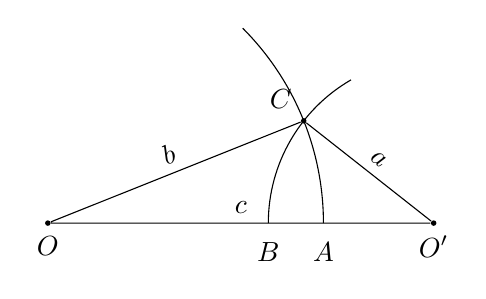
\begin{tikzpicture}[scale=.7]
	\node[circle, fill=black, inner sep=0pt, minimum size=2, label=below:{$O$}] (O) at (0,0) {};
	\node[circle, fill=black, inner sep=0pt, minimum size=2, label=below:{$O'$}] (P) at (7,0) {};
	\node[label=below:{$A$}] (A) at (5,0) {};
	\node[label=below:{$B$}] (B) at (4,0) {};
	\node[circle, fill=black, inner sep=0pt, minimum size=2, label=above left:{$C$}] (C) at ({acos((7-33/14)/5)}:5) {};
	\draw (B) arc (180:120:3) (A) arc (0:45:5);
	\draw (O) -- node[sloped, above]{$b$} (C) -- node[sloped, above]{$a$} (P) -- node[above]{$c$} (O);
\end{tikzpicture}
\caption{Construcción del triángulo en \ref{thm:triangle-side-construction}}
\end{figure}
\begin{cor}
Dada una longitud $s$, existe un triángulo equilatero de lado $s$.
\end{cor}
Cabe destacar que esta última es la primera construcción en \citetitle{euclides2007elements} de Euclides. Esto ofrece una comparación interesante, pues Euclides se interesaba en el como de las figuras, mientras que nosotros nos interesamos en el que de las mismas, en el si existen o no.

\textbf{La incertidumbre del criterio ALL.} Hemos visto como casi cualquier combinación entre lados y ángulos nos comprueba que dos triángulos son congruentes, sin embargo, la combinación ángulo-lado-lado es la única que puede generar incertidumbre. Para demostrar cómo, hemos de probar que existen dos triángulos que cumplirían con el criterio y que no son congruentes. Para ello consideremos un segmento $\overline{AB}$ cualquiera, un punto $D\in\overline{AB}$ y definamos a $\omega$ como la circunferencia de centro $B$ y radio $\overline{BD}$. Luego, sea $C_1$ uno de los dos puntos entre la intersección de $\omega$ y la perpendicular a $AB$ por $B$; entonces, $\angle AC_1B$ no puede ser recto, por el teorema~\ref{thm:triangle-ext-angle-bigger}, por lo que $AC_1$ es secante a $\omega$ y le corta en otro punto $C_2$. Finalmente, los triángulos $\triangle ABC_1$ y $\triangle ABC_2$ cumplen con los requisitos de un supuesto criterio ALL, pero resultan no ser congruentes.

\chapter{Geometría Euclídea}
Si hemos de hablar de matemática moderna no podemos dejar de lado a Euclides, quien con \textit{Los Elementos} formalizó por primera vez las matemáticas siendo él el primero en intentar crear un sistema axiomático sobre el cual resolvía problemas principalmente de índole de construcción. Mas es también importante apreciar que la visión que Euclides le da a la geometría difiere bastante de la nuestra, él se interesaba en como manualmente construir una figura (y más adelante, sobre construcciones de regla y compás veremos que clase de figuras se pueden obtener a partir únicamente de estas herramientas básicas), mientras que a nosotros nos interesa la cualidad de existencia, que es mucho más formalista.

Esta distinción es clave para comprender y distinguir entre lo que se denomina \textit{matemática clásica} y \textit{moderna} pues, y como puede ver, va mucho más allá de una simple convención temporal. Asimismo, cabe destacar que eventualmente veremos como poder aplicar otras ramas de las matemáticas (por lo que se recomiendan lecturas de otro tipo de textos), tales como el álgebra y el análisis, para profundizar y obtener nuevos resultados.

Además de ello, este capítulo ofrece algunos axiomas nuevos (el de Arquímedes, el de continuidad y el de Euclides) que ayudaran a obtener más resultados y obtener una visión más concisa sobre que tipo de geometría tratamos.

\section{Axioma de las paralelas}
\begin{mydef}[Paralelismo]
Diremos que dos rectas coplanares son \textit{paralelas}\index{paralelismo} syss son la misma o si no se intersectan. Así mismo lo son un par de planos. El paralelismo lo denotaremos como $a\parallel b$ en caso de las rectas y análogo en los otros casos.
\end{mydef}
\begin{prop}
Dada una recta (plano resp.), por un punto siempre pasa una recta (plano resp.) paralela a ésta.
\end{prop}
\begin{proof}
Llamemos $r$ a la recta y $P$ al punto. Primero construimos $s\perp r$ por $P$ (y llamamos $Q$ al pie de ésta) y luego $t\perp s$, también por $P$. Podemos comprobar que $r\parallel t$, pues de lo contrario se intersectarían en $R$ y $\triangle PQR$ tendría dos ángulos rectos lo que es imposible.

El argumento es análogo para los planos.
\end{proof}
\begin{axiom}[de las Paralelas (Euclides)]
Dada una recta, por un punto siempre pasa una única recta paralela a ésta.
\end{axiom}
\begin{cor}
Dado un plano, por un punto siempre pasa un único plano paralelo a este.
\end{cor}
\begin{proof}
Sea $\alpha$ el plano original y $P$ el punto elegido. Supongamos que $\beta_1$ y $\beta_2$ son paralelos a $\alpha$ por $P$, entonces $\beta_1$ y $\beta_2$ se intersectan en una recta $r$
\end{proof}
Consideremos dos rectas coplanares distintas $r_1,r_2$ y otra secante a ambas $s$ (si $r_1$ y $r_2$ se intersectan asumiremos que $s$ no les intersecta en ese mismo punto), tal como en la fig.~\ref{fig:alternated-angles} acontinuación. Diremos que los pares de ángulos 1 y 5, 2 y 6, 3 y 7, y 4 y 8 son \textbf{alternos}; que los pares de ángulos 3 y 6, y 4 y 5 son \textbf{alternos internos}; y que los pares de ángulos 1 y 8, y 2 y 7 son \textbf{alternos externos}.
\begin{figure}
\centering
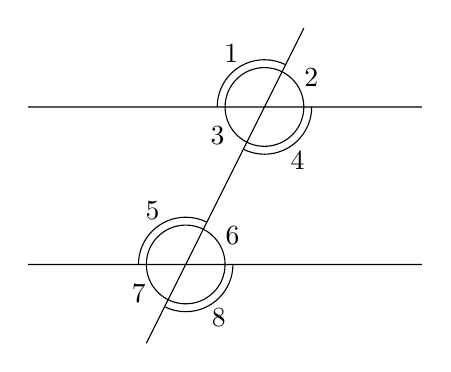
\begin{tikzpicture}
\draw (0,0) -- ++(5,0) (0,2) -- ++(5,0) (1.5,-1) -- ++(2,4);
\draw (3,2) circle (.5) (2,0) circle (.5) (3,2) ++(.6,0) arc (0:{atan(2)-180}:.6) (3,2) ++(-.6,0) arc (180:{atan(2)}:.6) (2,0) ++(.6,0) arc (0:{atan(2)-180}:.6) (2,0) ++(-.6,0) arc (180:{atan(2)}:.6);
\draw (3,2) +({atan(2)/2}:.7) node{2} +({(atan(2)+180)/2}:.8) node{1} +({180+atan(2)/2}:.7) node{3} +({270+atan(2)/2}:.8) node{4} (2,0) +({atan(2)/2}:.7) node{6} +({(atan(2)+180)/2}:.8) node{5} +({180+atan(2)/2}:.7) node{7} +({270+atan(2)/2}:.8) node{8};
\end{tikzpicture}
\caption{}\label{fig:alternated-angles}
\end{figure}
\begin{thm}\label{thm:parallel-cross}
Dada un par de rectas $r_1,r_2$ coplanares distintas cortadas por otra recta $s$, entonces, los ángulos alternos internos (y, por ende, los alternos externos también) son congruentes entre sí syss $r_1\parallel r_2$.
\end{thm}
\begin{proof}
Sean $A$ y $B$ los puntos de intersección entre $r_1$, y $r_2$ con $s$ resp.

$\implies$. Si $r_1$ y $r_2$ fuesen secantes, lo serían en $C$ con lo que formaríamos un triángulo tal que uno de los vértices tendría un ángulo suplementario igual a otro ángulo.

$\Longleftarrow$. Supongamos por contradicción que los ángulos alternos internos son distintos, entonces en el punto $A$ construimos una recta $r'$ tal que si cumple con que los ángulos alternos internos son iguales a los de $r_2$ con $s$ (esto al prolongar la semirrecta del axioma IV, 4). Luego $r'\parallel r_2$ por la parte ya probada. Finalmente, por el axioma de Euclides, $r_2=r'$.
\end{proof}
De ahora en adelante, admitiremos el convenio en que $\pi$ representa un ángulo llano, de manera que $\pi/2$ representa un ángulo recto.
\begin{thm}\label{thm:triangle-int-angle-sum}
La suma de ángulos internos de un triángulo es igual a $\pi$.
\end{thm}
\begin{proof}
Sea $\triangle ABC$ el triángulo, comenzaremos por construir una recta $r$ paralela a $AB$ por $C$. Luego el sistema $r,\,AB,\,AC$ corresponde al descrito en el teorema anterior, por lo que definiremos $P$ como aquél tal que $\angle CAB\equiv\angle PCA$ y, de manera análoga, deducimos que existe $Q$ tal que $P-C-Q$ y $\angle ABC\equiv\angle BCQ$. Finalmente, y por definición, $\angle A+\angle C+\angle B\equiv\angle PCA+\angle ACQ$, el cual es llano.
\end{proof}
\begin{figure}
\centering
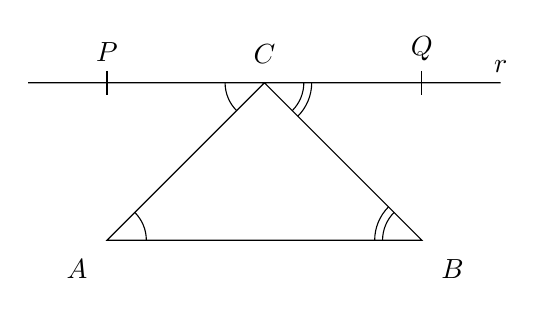
\begin{tikzpicture}
\node[label=below left:{$A$}] (A) at (0,0) {};
\node[label=below right:{$B$}] (B) at (4,0) {};
\node[label=above:{$C$}] (C) at (2,2) {};
\draw (A.center) -- (B.center) -- (C.center) -- cycle (C) +(-3,0) -- +(3,0) node[above]{$r$};
\draw (C) ++(-2,0) +(0,.15) node[above]{$P$} -- +(0,-.15) (C) ++(2,0) +(0,.15) node[above]{$Q$} -- +(0,-.15);
\draw (A) ++(.5,0) arc (0:45:.5) (C) ++(-.5,0) arc (180:225:.5) (B) ++(-.5,0) arc (180:135:.5) (B) ++ (-.6,0) arc (180:135:.6) (C) ++(.5,0) arc (0:-45:.5) (C) ++(.6,0) arc (0:-45:.6);
\end{tikzpicture}
\caption{Demostración del teorema~\ref{thm:triangle-int-angle-sum}}
\end{figure}
\begin{cor}
Dado $\triangle ABC$:
	\begin{enumerate}
		\item El ángulo externo a $C$ es igual a la suma de los otros dos ángulos internos, es decir, $\angle A + \angle B$.
		\item Si el triángulo es rectángulo en $C$ entonces $\angle A + \angle B \equiv \pi/2$.
		\item Si el triángulo es rectángulo en $C$ e isósceles, entonces $\angle A \equiv \angle B \equiv \pi/4$.
		\item Si el triángulo es equilatero, entonces todos sus ángulos (internos) miden $\pi/3$.
	\end{enumerate}
\end{cor}
\begin{mydef}[Paralelogramos]
Dados cuatro puntos distintos coplanares $A,\,B,\,C,\,D$ tales que $AB\parallel CD$ y $BC\parallel AD$, diremos que definen un \textit{paralelogramo}\index{paralelogramo} como el conjunto resultante de la intersección de los semiplanos de frontera alguna de las rectas $AB,\, BC,\, CD,\, DA$ que contiene a los puntos restantes. A los segmentos $\overline{AB}, \overline{BC}, \overline{CD}, \overline{DA}$ les llamaremos sus \textit{lados}, los ángulos $\angle ABC, \angle BCD, \angle CDA, \angle DAB$ son llamados sus \textit{ángulos internos}. Asimismo diremos que dos lados o ángulos son \textit{contiguos}\index{contiguos} syss comparten un punto en común, de lo contrario, diremos que son \textit{opuestos}. Los segmentos $\overline{AC}, \overline{BD}$ son llamados sus \textit{diagonales}.

Diremos que un paralelogramo es un \textit{rombo}\index{rombo} syss sus lados son todos congruentes entre sí. Diremos que un paralelogramo es un \textit{rectángulo}\index{rectángulo} si todos sus ángulos son congruentes entre sí. Diremos que un rombo es un \textit{cuadrado}\index{cuadrado} syss es también un rectángulo.
\end{mydef}
\begin{thm}
En un paralelogramo, sus lados y ángulos opuestos son congruentes entre sí; y sus ángulos contiguos son suplementarios. Las diagonales se cruzan en su punto medio.
\end{thm}
\begin{proof}
Las expresiones acerca de ángulos son consecuencia directa del teorema~\ref{thm:parallel-cross}, por lo que nos preocuparemos de las expresiones respecto de los lados. Para ello, vemos que $\triangle ACB\equiv\triangle CAD$ por ALA (los ángulos son congruentes por el teorema~\ref{thm:parallel-cross}).
\begin{figure}
\centering
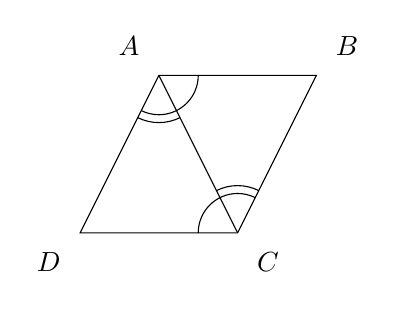
\begin{tikzpicture}
\node[label=above left:{$A$}] (A) at (1,2) {}; 
\node[label=above right:{$B$}] (B) at (3,2) {}; 
\node[label=below right:{$C$}] (C) at (2,0) {}; 
\node[label=below left:{$D$}] (D) at (0,0) {}; 
\draw (A.center) -- (B.center) -- (C.center) -- (D.center) -- cycle;
\draw (A.center) -- (C.center) (A.center) ++(.5,0) arc (0:{-90-atan(.5)}:.5) (A.center) ++({-atan(2)}:.6) arc ({-atan(2)}:{-90-atan(.5)}:.6) (C.center) ++(-.5,0) arc (180:{90-atan(.5)}:.5) (C.center) ++({180-atan(2)}:.6) arc ({180-atan(2)}:{90-atan(.5)}:.6);
\end{tikzpicture}
\caption{}
\end{figure}

La proposición de las diagonales se demuestra de la siguiente forma: primero vemos que han de intersectarse (digamos en $E$) puesto que $A$ y $D$ están en el mismo semiplano respecto a $BC$, luego $B$ y $D$ no pueden estar en el mismo semiplano respecto a $AC$ porque de lo contrario, $D$ estaría en el ángulo $\angle CAB$ por lo que, por el teorema de las barras cruzadas, las rectas no serían paralelos. Luego de deducir que se cortan, es facil probar que $\triangle EAB\equiv\triangle ECD$ por AAL.
\end{proof}
\begin{prop}
Un paralelogramo $ABCD$ es un rombo syss $AC\perp BD$.
\end{prop}
\begin{lem}\label{thm:lemma-for-thales}
Dados $s_1,s_2$ semirrectas con vértice común $O$, $P,Q$ en $s_1,s_2$ resp. distintos de $O$ y $A,B\in s_1$ distintos de $O$, tal que definimos $A',B'\in s_2$ como la intersección de $s_2$ y la paralela a $PQ$ que pasa por $A,B$ resp. Entonces la clase de congruencia de $\overline{A'B'}$ depende exclusivamente de la clase de congruencia de $\overline{AB}$.
\end{lem}
\begin{proof}
Sin perdida de generalidad asumamos que $O-A-B$ y llamemos $u:=\overline{AB}$. Supongamos que $C,D\in s_1$ también cumple que $\overline{CD}\equiv u$, entonces probaremos que $\overline{A'B'}\equiv\overline{C'D'}$. Para ello, definimos $R$ como la intersección entre la paralela a $s_2$ que pasa por $A$ y la paralela a $PQ$ que pasa por $B$. De ello definimos $R'$ análogamente para $C,D$. Es obvio que $AR_1B'A'$ es un paralelogramo, de forma que $\overline{A'B'}\equiv\overline{AR}$, y $\triangle ABR\equiv\triangle CDR$ (por ALA, por el teorema~\ref{thm:parallel-cross}).
\end{proof}
\begin{thm}[Propiedad de división de segmentos]
Dado un segmento $v$ y un número natural no nulo $n$ existe un segmento $u$ tal que $v\equiv nu$ (tal que denotaremos $u\equiv v/n$).
\end{thm}
\begin{proof}
Digamos que $v$ posee extremos $A$ y $B$, y sea $P$ un punto cualquiera no colinear. Tomando un segmento cualquiera $x$, existe $A_1\in\overrightarrow{AP}$ tal que $\overline{AA_1}\equiv x$, así mismo, construimos $A_2$ tal que $A-A_1-A_2$ y $\overline{A_1A_2}\equiv x$ y así sucesivamente hasta llegar a $A_n$. Luego, construimos $B_i$ como la intersección de la paralela a $A_nB$ que pasa por $A_i$ y $AB$, y definiremos $u:=\overline{AB_1}$. 
\begin{figure}
\centering
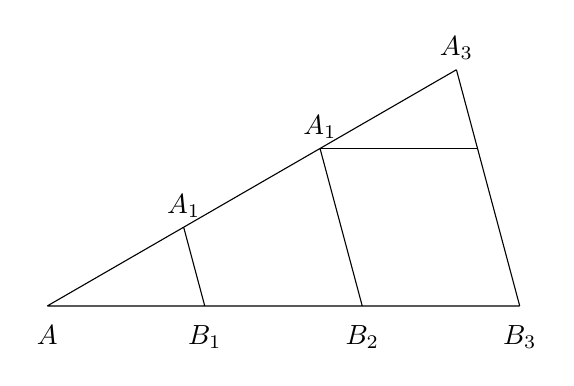
\begin{tikzpicture}[scale=2]
\node[label=below:{$A$}] (A) at (0,0) {}; 
\foreach \i in {1,2,3} {
\node (A\i) at (30:\i) {}; 
\node[label=below:{$B_\i$}] (B\i) at (\i,0) {}; 
}
\draw (A.center) -- node[sloped]{$\shortmid$} (A1.center) node[sloped,above]{$A_1$} -- node[sloped]{$\shortmid$} (A2.center) node[sloped,above]{$A_1$} -- node[sloped]{$\shortmid$} (A3.center) node[sloped,above]{$A_3$} (A.center) -- node[sloped]{$\shortparallel$} (B1.center) -- node[sloped]{$\shortparallel$} (B2.center) -- node[sloped]{$\shortparallel$} (B3.center) (A1.center) -- (B1.center) (A2.center) -- (B2.center) (A3.center) -- (B3.center);
\draw (A2.center) -- node[sloped]{$\shortparallel$} ++(1,0);
\end{tikzpicture}
\caption{}\label{fig:segment-division-euclid}
\end{figure}

	Por el lema anterior, para todo entero $1\leq i<n$, $\overline{B_iB_{i+1}}\equiv u$, por ende $v\equiv nu$ como se quería.
\end{proof}

\section{``Medida'' y Geometría Arquimediana}
No se puede hablar de ``medida'' de forma absoluta, sino que siempre se asocian números en comparación. Esto se evidencia en el campo de la física mediante lo que denominan ``unidades de medida''. Aún así, en esta sección, se pretende introducir el concepto de número mediante dicha comparación.
\begin{mydef}
Dado un número racional $r=n/m\in\Q$ positivo (con $n,m$ naturales) y un segmento $u$, denotaremos $ru$ como $n\cdot(u/m)$.
\end{mydef}
\begin{prop}
Dado un par de segmentos cualesquiera $u, v$ y un par de racionales $r, s\in\Q^+$, se cumple:
\begin{enumerate}
\item $(rs)u\equiv r(su)$.
\item $r(u+v)\equiv ru+rv$.
\item $(r+s)u\equiv ru+su$.
\item $1u\equiv u$.
\item Si $ru\equiv rv$, entonces $u\equiv v$.
\item Si $r<s$ entonces $ru< su$.
\item Si $u<v$ entonces $ru< rv$.
\end{enumerate}
\end{prop}
\begin{mydef}[Recta graduada]\index{recta!graduada}
Dados $P_0,P_1$ (en ese orden), definiremos $P_r$ con $r\in\Q$ de la siguiente manera: si $r>0$, entonces $P_r$ es el único punto de $\overrightarrow{P_0P_1}$ tal que $\overline{P_0P_r}\equiv r\overline{P_0P_1}$; si $r<0$, entonces $P_r$ es el único punto de la semirrecta complementaria a $\overrightarrow{P_0P_1}$ tal que $\overline{P_0P_r}\equiv (-r)\overline{P_0P_1}$.
\end{mydef}
Nótese que en la geometría euclídea automáticamente podemos construir un conjunto de números racionales para representar los puntos del espacio, pero una noción más relevante para los matemáticos es la de número real. Para ello, no hay ningún axioma que nos permita demostrar que existiendo $u$ exista $\sqrt[3]{2}u$\footnote{Demostrar la existencia de $\sqrt{2}$ por otro lado es bastante fácil con el teorema de Pitágoras que ya veremos más adelante.} por ejemplificar. Pero en primer lugar hemos de definir que significa ser un \textit{número real}.
\begin{mydef}[Orden en la recta]
Sea $AB$ una recta, entonces definiremos una relación $P<_{AB}Q$\nomenclature{$P<_{AB}Q$}{$P$ viene ántes que $Q$ en $AB$ (con ese sentido)} que habremos de interpretar como que desde $P$ hay que moverse en el mismo sentido que de $A$ a $B$ para llegar a $Q$. En particular definiremos las siguientes subrelaciones, considerando que $s:=\overrightarrow{AB}$:

Si $P, Q$ pertenecen a $s$, entonces
$$P<^+_{AB}Q\iff A-P-Q.$$
Si $P, Q$ pertenecen a la semirrecta complementaria de $s$ entonces
$$P<^-_{AB}Q\iff P-Q-A.$$
Entonces, definimos finalmente
$$P<_{AB}Q\iff\begin{cases}
P\notin s,Q\in s\\
P,Q\in s\wedge P<^+_{AB}Q\\
P,Q\notin s\wedge P<^-_{AB}Q
\end{cases}$$
\end{mydef}
\begin{thm}
Dada una recta $r$ con $A,B\in r$ distintos y $X,Y,Z\in r$, se cumple que:
\begin{enumerate}
\item La relación $\leq_{AB}$ es de orden total en $r$ (el orden total implica comparabilidad, es decir, que siempre o $X\leq_{AB}Y$ o $Y\leq_{AB}X$).
\item $A<_{AB}B$.
\item $\leq_{AB}$ equivale a $\leq_{XY}$ syss $X<_{AB}Y$.
\item $X-Y-Z$ syss $X<_{AB}Y<_{AB}Z$ ó $Z<_{AB}Y<_{AB}X$.
\end{enumerate}
\end{thm}
\begin{proof}
Todas las expresiones o son triviales, o se desprenden del segundo teorema de Pasch (mediante estudio de casos particulares), o son consecuencia de una definición (la comparabilidad se deriva del concepto de ``semirrecta'').
\end{proof}
\begin{mydef}[Corte o partidura]
Dado un punto $P$ en una recta graduada, definimos el siguiente conjunto como un corte o partidura de la recta:
$$\alpha_P:=\{r\in\Q:P_r<P\}$$
Asimismo, diremos que un conjunto $\alpha$ es una sección abierta de $\Q$ syss cumple ser:
\begin{enumerate}[$a)$]
\item $x\in\Q$ e $y<x$ implica $y\in\alpha$.
\item Para todo $x\in\Q$ existe $y\in\alpha$ tal que $x<y$.
\end{enumerate}
\end{mydef}
\begin{mydef}[Proporción de segmentos]
Dados dos segmentos $u,v$, dos puntos distintos $P_0,Q$, definiremos $P_1$ y a $P$ como el único par de puntos de $\overrightarrow{P_0Q}$ tal que $\overline{P_0P_1}\equiv u$ y que $\overline{P_0P}\equiv v$ resp. Luego, definimos su proporción, como
$$\frac{v}{u}:=\alpha_P$$
\end{mydef}
La idea de los cortes en la recta graduada es que todo segmento tiene un corte asociado, sin embargo, nuestra definición de sección abierta admite los conjuntos $\emptyset,\Q$ a los cuales no podríamos admitir puntos, pues serían los más alejados en ambas semirrectas.
\begin{mydef}[Conjunto de números reales $\R$]
Diremos que existe un conjunto descrito como $\overline{\R}$ tal que contiene a todas las secciones abiertas de $\Q$. Admitiendo la notación de que $-\infty:=\emptyset$ y que $+\infty:=\Q$, definimos $\R:=\overline{\R}\setminus\{\pm\infty\}$ tal que sus elementos serán llamados \textit{números reales}\index{numero@número!real}.
\end{mydef}
Cabe destacar que esta construcción de los reales corresponde a la descrita como los ``cortes de Dedekind'' (aunque adaptada para el contexto geométrico del libro).
\begin{prop}
Los conjuntos $\R$ y $\overline{\R}$ son totalmente ordenado bajo la relación $\subseteq$. El primero no tiene máximo ni mínimo, mientras que el segundo si lo poseen y son $+\infty$ y $-\infty$ resp.
\end{prop}
\begin{proof}
Es evidente que $\subseteq$ constituye un orden parcial en cualquier familia de conjuntos, mas es de orden total pues suponiendo que $\alpha,\beta\in\R$ y, sin perdida de generalidad, que $b\in\beta\setminus\alpha$, entonces para cualquier $a\in\alpha$ se debe dar que $a<b$ (de lo contrario $b\in\alpha$), por ende, $\alpha\subset\beta$.

Respecto a lo de los máximos y mínimos es evidente que todo $\alpha\in\overline{\R}$ satisface que $\emptyset\leq\alpha\leq\Q$ (por definición). Mientras que si $\alpha\in\R$, entonces no puede ser $\Q$ por ende existe $b\in\Q\setminus\alpha$, luego $\beta=\{r\in\Q:r<b+1\}$ cumple que $\alpha<\beta$. Asimismo, $\alpha\neq\emptyset$, luego $a\in\alpha$, por ende, existe $\gamma=\{r\in\Q:r<a\}\in\R$ tal que $\gamma<\alpha$.
\end{proof}
\begin{mydef}[Supremo e ínfimo]
	Sea $A$ un subconjunto de $X$ un conjunto parcialmente ordenado. Si $A$ es acotado\footnote{Diremos que $x$ es una cota superior (resp. inferior) si para todo $a\in A$ se da que $a\leq x$ (resp. $x\leq a$).}, entonces diremos que posee supremo\index{supremo} (resp. ínfimo\index{infimo@ínfimo}) $s$ si para toda cota superior (resp. inferior) $c$ se da que $s\leq c$ (resp. $c\leq s$).
\end{mydef}
Cabe destacar que si un conjunto posee máximo (resp. mínimo) ese corresponde a su supremo (resp. mínimo). Lo que se debe comprender de los supremos e ínfimos es que no son necesariamente elementos del conjunto. Además, por ser $X$ ordenado, comprendemos que de existir, el supremo e ínfimo son únicos.
\begin{thm}
Se da que:
\begin{enumerate}
\item Todo subconjunto de $\overline{\R}$ posee supremo e ínfimo.
\item Todo subconjunto no vacío de $\R$ acotado superiormente (resp. inferiormente) posee supremo (resp. ínfimo).
\end{enumerate}
\end{thm}
\begin{proof}
\begin{enumerate}
\item Consideremos $X\subseteq\R$, entonces su supremo es
$$\bigcup_{\alpha\in X}\alpha$$
y su ínfimo es el supremo del conjunto de cotas inferiores.
\item Supongamos que $c$ es una cota superior, entonces el conjunto $M:=\bigcup_{\alpha\in X}\alpha$ no puede ser $+\infty$, pues no ha de contener a $c$, tampoco ha de ser $-\infty$ pues es no vacío. Es análogo para el ínfimo.
\end{enumerate}
\end{proof}
\begin{prop}\label{thm:rational-inclusion-reals}
Sea $P\in r$ donde $r$ es una recta graduada, entonces las aplicaciones $i:r\rightarrow\R$ con $i(P)=\alpha_P$ y $j:\Q\rightarrow\R$ con $j(q)=\{t\in\Q:t<q\}$ son inyectivas.
\end{prop}
\begin{mydef}
Dado $x\in\R$, denotaremos $P_x$ al único punto (si existe) que satisface que $\alpha_{P_x}=x$. Luego, por definición (de Dedekind) de los números reales sigue que
$$\frac{\overline{P_0P_{\pm x}}}{P_0P_1}=x$$
o también, lo denotaremos como que $\overline{P_0P_{\pm x}}\equiv x\overline{P_0P_1}$.
\end{mydef}
\begin{mydef}[Operaciones en $\R$]
Sean $x,y\in\R$, denotamos
	$$x+y=\sup\{r+s:r\in x,s\in y\},$$
y también
	$$-x=\sup\{-r:r\in\Q,x<r\}.$$
Sean $x,y>0$, entonces, denotamos
	$$xy=\sup\{rs:r\in x,s\in y;0<r,s\}$$
Más generalmente:
	$$xy=\begin{cases}
	-(-x)y, &x<0,y>0\\
	-x(-y), &x>0,y<0\\
	(-x)(-y), &x<0,y<0
	\end{cases}$$
\end{mydef}
\begin{thm}
$(\R,+,\cdot)$ es un cuerpo con neutro de $+$ el 0 y neutro de $\cdot$ el 1. Asimismo, la aplicación $j$ de la proposición~\ref{thm:rational-inclusion-reals} es un epimorfismo de cuerpos.
\end{thm}
\begin{proof}
Es fácil comprobar la asociatividad, conmutatividad, existencia del elemento neutro y de los opuestos considerando que $x\leq y$ con $x,y\in\R$ syss $r<y\implies r<x$ con $r\in\Q$ (por ende, $r<x\iff r<y$ significa que $x=y$).

Es inmediato comprobar la asociatividad, conmutatividad y que 1 es el neutro del producto. El inverso, para $x>0$ se define como
	$$x^{-1}:=\sup\{r^{-1}:r\in\Q,0<r<x\},$$
y si $x<0$, entonces $x^{-1}:=-(-x)^{-1}$. Con esta definición, es también fácil ver que efectivamente son inversos.
\end{proof}
\begin{thm}
Sea $\mu$ una aplicación (que llamaremos ``medida aditiva'')\index{medida aditiva} desde el conjunto de segmentos al de números reales tal que
\begin{enumerate}[$a)$]
	\item $u\equiv v\implies \mu(u)=\mu(v)$.
	\item $\mu(u+v)=\mu(u)+\mu(v)$.
\end{enumerate}
Entonces, para todo par de segmentos $u,v$ se da que
$$\frac{\mu(u)}{\mu(v)}=\frac{u}{v}$$
\end{thm}
\begin{proof}
Sea $q$ un natural no nulo, entonces $\mu(qx)=q\mu(x)$, es decir, definiendo $u\equiv qx$, nos queda
$$\frac{\mu(u/q)}{\mu(u)}=\frac{1}{q}.$$
Sea $p$ otro natural no nulo y definiendo $r:=p/q\in\Q^+$, entonces
$$\frac{\mu(ru)}{\mu(u)}=r.$$
Sea $\alpha\in\R^+$ tal que $r,s\in\Q^+$ satisfacen que $r<\alpha<s$, como $x<y$ implica $y\equiv x+z$, luego $\mu(x)<\mu(x)+\mu(z)=\mu(y)$. Por ende,
$$r=\frac{\mu(ru)}{\mu(u)}<\frac{\mu(\alpha u)}{\mu(u)}<\frac{\mu(su)}{\mu(u)}=s,$$
es decir, $\mu(\alpha u)/\mu(u)=\alpha$. Sustituya $v\equiv\alpha u$ y está completo.
\end{proof}
\begin{mydef}[Triángulos similares]
Denotaremos $\triangle ABC\sim\triangle A'B'C'$\nomenclature{$\sim$}{Tales figuras son similares} (léase ``$\triangle ABC$ y $\triangle A'B'C'$ son \textit{similares}\index{similares!(triángulos)} en ese orden'') syss sus lados son proporcionales dos a dos, es decir,
$$\frac{AB}{AB'}=\frac{AC}{AC'}=\frac{BC}{B'C'}.$$
\end{mydef}
\begin{thm}[Teorema de Tales]\index{teorema!de Tales}
Dados $\triangle ABC$ y $\triangle AB'C'$ tales que $B'\in\overrightarrow{AB}$, $C'\in\overrightarrow{AC}$ y que $BC\parallel B'C'$. Entonces $\triangle ABC\sim\triangle AB'C'$. 
\end{thm}
\begin{proof}
Nótese que por el lema~\ref{thm:lemma-for-thales}, la clase de congruencia de $\overline{AC}$ sólo depende de $\overline{AB}$, por ende, dados un segmento $u$ arbitrario, definiremos $m$ como la función tal que con $P,Q\in\overrightarrow{AB}$ y $P'Q'\in\overrightarrow{AC}$ segun la construcción del mismo lema se cumpla $\overline{P'Q'}\equiv m(\overline{PQ})u$. Es inmediato ver que dicha función es una medida aditiva. En particular, como el valor es un real positivo, existe su inverso multiplicativo, por ende, mediante igualdades se llega a la primera proporción (de los lados $\overline{AB}$ con $\overline{AC}$). La proporción restante es análoga.
\end{proof}
\begin{thm}
Todo par de triángulos cuyos respectivos ángulos son congruentes resultan ser semejantes.
\end{thm}
\begin{cor}
Un triángulo es equilatero syss posee los tres ángulos congruentes entre sí.
\end{cor}
\begin{thm}
Un par de triángulos son semejantes syss poseen un ángulo congruente y el par de lados adyacentes proporcionales.
\end{thm}
\begin{proof}
Para la prueba, se construye un triángulo con dichas características que resulte ser semejante y se comprueba que es congruente al triángulo descrito en la expresión.
\end{proof}
\begin{thm}[Teorema de Pitágoras]\index{teorema!de Pitágoras}
En un triángulo rectángulo el cuadrado de la hipotenusa es igual a la suma de los catetos al cuadrado.
\end{thm}
\begin{proof}
Digamos que el triángulo posee vértices $A,B,C$ cuyos lados son $a,b,c$, cada uno tomando el nombre según el vértice opuesto y tal que el ángulo recto es $\angle C$ (por ende, $c$ es la hipotenusa). Definimos $D$ como el pie de la perpendicular a $AB$ por $C$.
\begin{figure}
\centering
\begin{tikzpicture}[scale=1.5]
	\node[label=below left:{$A$}] (A) at (0,0) {};
	\node[label=above:{$C$}] (C) at (60:{sqrt(3)}) {};
	\node[label=below:{$D$}] (D) at ($(C)+(0,-1.5)$) {};
	\node[label=below right:{$B$}] (B) at ($(C)+(-30:3)$) {};
	\draw (A.center) -- (B.center) -- (C.center) -- cycle;
	\draw (A.center) ++(.25,0) arc (0:60:.25) (C.center) ++(-30:.25) arc (-30:-120:.25) (C.center) ++(-90:.3) arc (-90:-120:.3) (B.center) ++(-.25,0) arc (180:150:.25) (B.center) ++(-.3,0) arc (180:150:.3);
	\draw (C.center) -- (D.center) +(-.125,0) rectangle +(.125,.125);
\end{tikzpicture}
\caption{}
\end{figure}

Para comprobar que $A-D-B$ comenzaremos por definir $E$ tal que $D-C-E$, tal que como $\angle ABE\equiv\angle ABC+\angle CBE$ se comprueba que $\overrightarrow{BC}\subset\angle ABE$ y por el teorema de las barras cruzadas, intersecta a $\overline{AE}$ digamos en $F$. Luego $DC$ intersecta a $\overline{FB}$, pero no a $\overline{AF}$ (pues intersecta su prolongación en $E$), por lo tanto, por el axioma de Pasch, intersecta a $\overline{AB}$ y ha de ser en $D$.

Luego, es fácil comprobar que $\triangle ADC\sim\triangle CDB\sim\triangle ACB$. De lo que podemos extraer las siguientes proporciones:
$$\frac{a}{\overline{BD}}=\frac{c}{a},\quad\frac{b}{\overline{DA}}=\frac{c}{b}$$
De lo que se concluye que
$$a^2+b^2=c\cdot\overline{BD}+c\cdot\overline{DA}=c(\overline{BD}+\overline{DA})=c^2.$$
\end{proof}
\begin{axiom}[de la propiedad Arquimediana]\index{propiedad!arquimediana}
	Dados $u,v$, existe $n$ natural tal que $v<nu$.
\end{axiom}

\section{Arcos, ángulos y cuerdas}
Cabe destacarse que el mayor de los problemas que podría encontrar un lector que desconozca el análisis matemático en esta sección es que, a diferencia de los segmentos, los ángulos no pueden ser divididos con nuestros axiomas en un natural $n$ cualquiera. No obstante, pueden ser divididos en dos, lo que implica que existiendo un ángulo $\theta$ existe $\theta/2^n$ con $n$ natural. Igualmente, nos las arreglaremos para introducir a los reales, pese a nuestras restricciones. Otra observación es que es gracias al axioma de las paralelas que se nos permite la división de segmentos, mas se puede prescindir de él del mismo modo que haremos en esta sección.
\begin{thm}[Propiedad Arquimediana (Ángulos)]
Dados un par de ángulos $\theta,\phi$ existe $n$ natural tal que $n\theta$ no está definido o $\phi<n\theta$.
\end{thm}
Cabe destacar que el subconjunto determinado por
$$\Q_2:=\left\{\frac{n}{2^m}:n,m\in\N\right\}$$
es un subcuerpo de $(\Q,+,\cdot)$ cuyos elementos llamaremos \textit{racionales diádicos}\index{numero@número!racional diádico}.
\begin{thm}
Sean $\alpha,\beta,\gamma$ ángulos cualesquiera:
\begin{enumerate}
	\item Existe $\pi\geq 1$ real tal que para todo racional diádico positivo $r$ existe (o está definido) el ángulo $r\alpha$.
	\item Existe un racional diádico $r$ tal que si $\alpha<\gamma$, entonces $\alpha<r\beta<\gamma$.
\end{enumerate}
\end{thm}
\begin{proof}
\begin{enumerate}
	\item Sabemos que $r=1$ pertenece al conjunto de los racionales diádicos tales que $r\alpha$ está definido. Asimismo, la propiedad arquimediana angular sugiere que existe una cota superior natural, por ende, como el conjunto es no vacío y acotado superiormente, entonces definimos $\pi$ como su supremo.
	\item Por propiedad arquimediana, sabemos que existe $n\in\N$ tal que $\beta<n(\gamma-\alpha)$, como\footnote{No hemos probado esta proposición, pero es una inmediata aplicación de la propiedad de inducción descrita en [TdC].} $n<2^n$ nos queda que $\beta/2^n<\gamma-\alpha$. Así mismo, elegimos a $m\in\N$ como el menor natural tal que $\alpha<m(\beta/2^n)$, de forma que $(m-1)(\beta/2^n)\leq\alpha$. Por lo tanto, se concluye que
		$$\frac{m}{2^n}\beta\equiv\frac{m-1}{2^n}\beta+\frac{1}{2^n}\beta<\alpha+(\gamma-\alpha)\equiv\gamma,$$
	con lo que el teorema queda probado.
\end{enumerate}
\end{proof}
Cabe destacar que, de ahora en adelante, admitiremos la notación de que $\pi$ representa el ángulo llano (o, en otras palabras, que $\pi/2$ es el ángulo recto).
\begin{mydef}
	Sea $\omega$ una circunferencia, diremos que un ángulo está \textit{inscrito en ella}\index{angulo@ángulo!inscrito en una circunferencia} syss su vértice pertenece a $\omega$ y sus lados no son tangentes a $\omega$.

	Asimismo, con la notación de que $A$ y $B$ son las otras intersecciones de las rectas con $\omega$ y que $O$ es su centro, llamamos el \textit{arco abarcado} por dichas rectas, lo que denotamos como $\overarc{AB}$ al ángulo $\angle AOB$.
\end{mydef}
\begin{thm}[Teorema del ángulo inscrito]\index{teorema!del ángulo inscrito}
	Dada una cuerda $\overline{AB}$ en una circunferencia $\omega$ que no es un diámetro, y un punto $C\in\omega$ contenido en el mismo semiplano de frontera $AB$ que contiene a su centro. Se da que $\overarc{AB}\equiv 2\angle ACB$.
\end{thm}
\begin{proof}
Denotaremos $\alpha:=\angle ACB$, $O$ al centro de $\omega$ y separaremos la demostración en tres casos:
\begin{description}
	\item[$O\in CA\cup CB$:] Sin perdida de generalidad asumimos que $C-O-A$. Luego, como $\triangle COB$ es isósceles con base $\overline{BC}$, se da que $\angle OBC\equiv\angle BCO$. Y como $\angle AOB$ es suplementario a $\angle COB$ se da la relación buscada.
	\item[$O\in\angle ACB$:] Llamemos $D$ a la intersección restante de $\omega$ con $CO$ (pues $C$ ya es una de las dos). Luego, por la propiedad anterior se ve que $\angle DOA\equiv2\angle DCA$ (análogo con $B$), por lo que
	\begin{align*}
		\angle AOB&\equiv\angle AOD+\angle DOB\equiv2\angle ACD+2\angle DCB\\
		&\equiv 2(\angle ACD+\angle DCB)\equiv 2\angle ACB
	\end{align*}
\item[$O\notin\angle ACB$:] Llamemos $\alpha:=\angle ACO$ y $\beta:=\angle BCO$, y $D$ a la intersección restante entre $\omega$ y $CO$. Entonces, por la primera demostración, se cumple que $\angle AOD\equiv2\alpha$ y $\angle BOD\equiv2\beta$ (ver fig.~\ref{fig:angle-arc-difference}).
	\begin{figure}
	\centering
	\begin{tikzpicture}
		\node[label=above:{$O$}] (O) at (0,0) {};
		\node[label=below left:{$A$}] (A) at (-120:2) {};
		\node[label=below right:{$B$}] (B) at (-60:2) {};
		\node[label=above left:{$C$}] (C) at (150:2) {};
		\node[label=below right:{$D$}] (D) at (-30:2) {};
		\draw (A.center) -- node[sloped]{$\shortmid$} (O.center) -- node[sloped]{$\shortmid$} (B.center);
		\filldraw[nicered,draw=black] (O.center) -- +(-30:.7) arc (-30:-60:.7) -- cycle;
		\filldraw[niceblue,draw=black] (O.center) -- +(-30:.5) arc (-30:-120:.5) -- cycle;
		\draw (O.center) circle (2) (D.center) -- (O.center) -- node[sloped]{$\shortmid$} (C.center) -- (A.center) -- (B.center) -- (C.center);
		\filldraw[nicered!50,draw=black] (C.center) -- +(-30:.7) arc (-30:-45:.7) -- cycle;
		\filldraw[nicered!50,draw=black] (B.center) -- +(120:.7) arc (120:135:.7) -- cycle;
		\filldraw[niceblue!50,draw=black] (C.center) -- +(-30:.5) arc (-30:-75:.5) -- cycle;
		\filldraw[niceblue!50,draw=black] (A.center) -- +(60:.5) arc (60:105:.5) -- cycle;
	\end{tikzpicture}
		\caption{}\label{fig:angle-arc-difference}
	\end{figure}

	Luego, se debe dar que $A,O$ están en semiplanos opuestos relativo a $BC$ o que $B,O$ están en semiplanos opuestos relativo a $AC$. Sin perdida de generalidad, supondremos la primera, con lo que construimos $E$ como la intersección de $\overline{AO}$ con $\overline{BC}$. De esto se concluye que $\beta<\alpha$ y que $\angle ACB\equiv\alpha-\beta$. Finalmente
	$$\angle AOB\equiv2\alpha-2\beta\equiv2(\alpha-\beta)\equiv2\angle ACB.$$
\end{description}
\end{proof}
\begin{cor}
Dos ángulos inscritos en una circunferencia son congruentes si abarcan el mismo arco.
\end{cor}
\begin{cor}
	Sea $\overline{AB}$ un diámetro de una circunferencia $\omega$ y $C\in\omega$ distinto a $A,B$; entonces $\angle ACB\equiv\pi/2$.
\end{cor}
\begin{cor}
	Un paralelogramo $ABCD$ es un rectángulo syss $\overline{AC}\equiv\overline{BD}$.
\end{cor}
\begin{proof}
	Sabemos que en un paralelogramo, las diagonales se intersectan en un punto $O$ que resulta ser punto medio de ambas, por lo que $r:=\overline{OA}\equiv\overline{OB}\equiv\overline{OC}\equiv\overline{OD}$. Luego sea $\omega$ la circunferencia de centro $O$ y radio $r$, entonces, $A,B\in\omega$ y, por lo tanto, $\angle DAB\equiv\angle ABC\equiv\pi/2$ por el corolario anterior.
\end{proof}
\begin{figure}
	\centering
	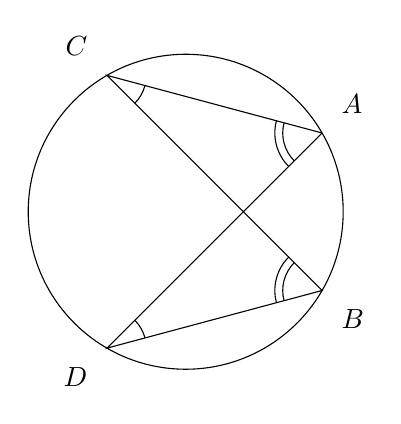
\begin{tikzpicture}
		\node[label=above right:{$A$}] (A) at (30:2) {};
		\node[label=below right:{$B$}] (B) at (-30:2) {};
		\node[label=above left:{$C$}] (C) at (120:2) {};
		\node[label=below left:{$D$}] (D) at (-120:2) {};
		\draw (0,0) circle (2) (A.center) -- (C.center) -- (B.center) -- (D.center) -- (A.center);
		\draw (C.center) ++(-15:.5) arc (-15:-45:.5) (D.center) ++(15:.5) arc (15:45:.5) (A.center) ++(165:.5) arc (165:225:.5) (A.center) ++(165:.6) arc (165:225:.6) (B.center) ++(135:.5) arc (135:195:.5) (B.center) ++(135:.6) arc (135:195:.6);
	\end{tikzpicture}
	\caption{}
	\label{fig:inscribed-arc-equity}
\end{figure}
\begin{thm}
	Dadas dos rectas secantes que se intersectan entre sí y con una circunferencia, tal que su intersección es interna a ella. Entonces, el ángulo en dicho punto es la semisuma\footnote{Diremos \textit{semisuma} (resp. \textit{semirresta}) al acto de sumar (resp. restar) dos valores, todo dividido en dos.} de los arcos que abarca.
\end{thm}
\begin{proof}
	Considere la situación descrita en la fig.~\ref{fig:inscribed-arc-equity} tal que $\alpha:=\angle ACB$ y $\beta:=\angle CAD$. Luego, como el ángulo externo de un triángulo es la suma de los dos restantes se da el teorema (sabiendo también que $\overarc{AB}\equiv 2\alpha$).
\end{proof}
\begin{thm}
	Dadas dos rectas secantes entre sí y con una circunferencia, tal que su intersección es externa a la circunferencia. Entonces el ángulo en dicho punto es la semirresta de los arcos que abarca.
\end{thm}
\begin{proof}
	Llamemos $P$ su intersección y supongamos la situación del teorema anterior, luego $\angle DAP\equiv\angle CBP\equiv\pi-\alpha$. Llamemos $x:=\angle DAB$ y $x':=\angle BAP$, y análogo con $y,y'$. Luego, por definición, $x+x'\equiv y+y'\equiv\pi-\alpha$. Así como que $x+y\equiv\pi-(\alpha+\beta)$ y que $\angle APB\equiv\pi-(x'+y')$. Finalmente,
		$$x'+y'\equiv2(\pi-\alpha)-(x+y)\equiv\pi-(\alpha-\beta).$$
\end{proof}
\begin{prop}
Sean $A, B, C$ puntos distintos de una circunferencia $\omega$ tal que $C$ está en el mismo semiplano de frontera $AB$ que contiene al centro de $\omega$ y tal que $l$, que contiene a $A$, es tangente a $\omega$. Entonces, con $Q \in l$ en el semiplano opuesto a $C$ relativo a $AB$, $\angle BAQ \equiv \angle ACB$.
\end{prop}
\begin{proof}
	Sea $D \in \omega$ tal que $\overline{AD}$ es un diámetro y definamos que $\theta := \angle ADB$, así como también que $P$ es la intersección entre $DB$ y $l$. Sabemos que $\angle ABD \equiv \pi/2 \equiv \angle DAP$, por lo tanto, $\angle BAD \equiv \angle AP D$ (pues comparten un ángulo y la suma es siempre la misma), con lo que $\angle BAP \equiv \angle ADB \equiv \theta$ que es congruente a $\angle ACB$ pues abarcan el mismo arco (ver fig.~\ref{fig:tangent-angle-equal-inscribed}).
\end{proof}
\begin{figure}
	\centering
	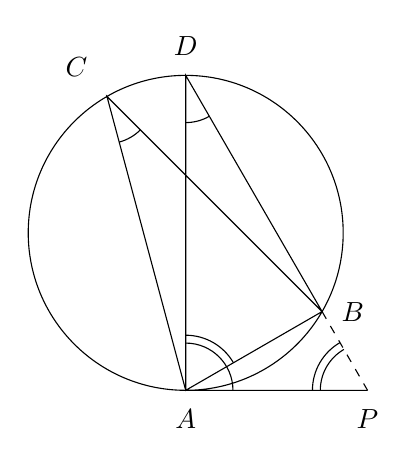
\begin{tikzpicture}[scale=2]
		\node[label=below:{$A$}] (A) at (-90:1) {};
		\node[label=right:{$B$}] (B) at (-30:1) {};
		\node[label=above left:{$C$}] (C) at (120:1) {};
		\node[label=above:{$D$}] (D) at (90:1) {};
		\node[label=below:{$P$}] (P) at ({sqrt(4/3)},-1) {};
		\draw (0,0) circle (1) (P.center) -- (A.center) -- (C.center) -- (B.center) -- (A.center) -- (D.center) -- (B.center);
		\draw[dashed] (B.center) -- (P.center);
		\draw (A.center) ++(.3,0) arc (0:90:.3) (A.center) ++(30:.35) arc (30:90:.35) (C.center) ++(-45:.3) arc (-45:-75:.3) (D.center) ++(-60:.3) arc (-60:-90:.3) (P.center) ++(-.3,0) arc (180:120:.3) (P.center) ++(-.35,0) arc (180:120:.35);
	\end{tikzpicture}
	\caption{}\label{fig:tangent-angle-equal-inscribed}
\end{figure}
\begin{prop}
Dado un triángulo $\angle ABC$, una circunferencia $\omega$ y un punto $A'\in\omega$, existen $A',B'\in\omega$ tales que $\triangle ABC\sim\triangle A'B'C'$.
\end{prop}
\begin{proof}
	Sea $r$ la recta tangente a $\omega$ en $A'$ y sea $P\in r$ distinto de $A'$ y en el semiplano de frontera $r$ que contiene a $O$ construimos $s_1$ tal que $\angle(\overrightarrow{A'P},s_1)\equiv\angle C$. Como esta recta es secante a $\omega$ y le intersecta en $A'$, diremos que su otra intersección es $B'$. Luego, construimos $s_2$ en el semiplano de frontera $A'B'$ que no contiene a $P$ tal que $\angle(s_1,s_2)\equiv\angle A$ y por el mismo argumento denotamos $C'$ a la intersección restante entre $s_2$ y $\omega$. Por la propiedad anterior se comprueba que $\angle A'C'B'\equiv\angle PA'B'\equiv\angle C$, y como poseen dos ángulos congruentes dos a dos son similares (ver fig.~\ref{fig:inscribed-similar-triangles}).
\end{proof}
\begin{figure}
	\centering
	\begin{tikzpicture}[scale=2]
		\node[label=below:{$A'$}] (A') at (-90:1) {};
		\node[label=right:{$B'$}] (B') at (-30:1) {};
		\node[label=left:{$C'$}] (C') at (150:1) {};
		\node[label=left:{$C$}] (C) at (2,0) {};
		\node[label=right:{$B$}] (B) at ($(C)+(15:2)$) {};
		\node[label=above:{$A$}] (A) at ($(B)+(135:1)$) {};
		\fill[niceblue!75] (A'.center) -- ++(.3,0) arc (0:30:.3) -- (A'.center) (C.center) -- ++(15:.3) arc (15:45:.3) -- (C.center) (C'.center) -- ++(-30:.3) arc (-30:-60:.3) -- (C'.center);
		\fill[nicegreen!75] (A'.center) -- ++(30:.3) arc (30:120:.3) -- (A'.center) (A.center) -- ++(-45:.3) arc (-45:-135:.3) -- (A.center);
		\fill[nicered!75] (A'.center) -- ++(120:.3) arc (120:180:.3) -- (A'.center) (B.center) -- ++(135:.3) arc (135:195:.3) -- (B.center) (B'.center) -- ++(150:.3) arc (150:210:.3) -- (B'.center);
		\draw (0,0) circle (1) (A'.center) +(1.2,0) node[right]{$r$} -- +(-1.2,0) (A'.center) -- (B'.center) -- (C'.center) -- (A'.center);
		\draw (A.center) -- (B.center) -- (C.center) -- cycle;
		\draw[dashed] (B'.center) -- +(30:.5) node[above right]{$s_1$} (C'.center) -- +(120:.5) node[above left]{$s_2$};
	\end{tikzpicture}
	\caption{}\label{fig:inscribed-similar-triangles}
\end{figure}
\begin{thm}
	Sean $\overline{AB}$ y $\overline{CD}$ cuerdas en $\omega$ que se intersectan en $P$, entonces
	$$\overline{AP}\cdot\overline{PB}\equiv\overline{CP}\cdot\overline{PD}.$$
\end{thm}
\begin{proof}
Para probarlo, basta con ver que $\triangle APC\sim\triangle DPB$ y, seguido aplicar el teorema de Tales.
\end{proof}
\begin{thm}
Sea $P$ un punto externo a una circunferencia $\omega$ tal que $PO$ intersecta a $\omega$ en $A,B$ y tal que existe $Q\in\omega$ tal que $PQ$ es tangente a $\omega$. Entonces
	$$\overline{AP}\,\overline{BP}=\overline{PQ}^2.$$
\end{thm}
\begin{proof}
	Supongamos que $P-O-A$ (con lo que $P-B-A$), luego
	$$\overline{OP}^2=(\overline{OB}+\overline{BP})^2=\overline{OB}^2+2\overline{OB}\,\overline{BP}+\overline{BP}^2,$$
	cabe destacar que $\overline{AB}\equiv 2\overline{OB}$.

	Asimismo, como $PQ$ es tangente a $\omega$ por $Q$, se tiene que $\triangle POQ$ es rectángulo en $Q$. Por teorema de Pitágoras
	$$\overline{OP}^2=\overline{PQ}^2+\overline{OQ}^2.$$
	Utilizando ambas expresiones y recordando que por definición de círculo, se da que $\overline{OQ}\equiv\overline{OB}$, por lo que, cancelando, queda
	$$\overline{PQ}^2=\overline{BP}^2+\overline{AB}\,\overline{BP}=(\overline{AB}+\overline{BP})\overline{BP}=\overline{AP}\,\overline{BP}.$$
\end{proof}
\begin{thm}
	Dado un par de rectas secantes entre sí en $P$ y a una circunferencia en los puntos $A,B$ (la primera), $C,D$ (la segunda). Entonces
	$$\overline{AP}\cdot\overline{BP}=\overline{CP}\cdot\overline{DP}.$$
\end{thm}

\section{Trigonometría}
Por el teorema de Tales, sabemos que existe una relación entre las medidas de los lados de un triángulo cuando sus ángulos son congruentes dos a dos, por lo tanto, es lógico que dados sus valores y un lado podamos deducir cuando miden los otros dos, mas no conocemos técnica alguna que nos sirva en este caso. Es ahí donde entra la \textit{trigonometría}\footnote{Del gr. ``medida de triángulos''.}; si bien en este capítulo no se enseñará un método exacto de cálculo, sí se repasarán teoremas involucrando tales técnicas.
\begin{mydef}[Funciones o razones trigonométricas]
	Dado $\triangle ABC$ rectángulo en $C$, definiremos $\sin,\cos$ (léanse ``seno'' y ``coseno'' resp.) como funciones cuyo dominio son las clases de congruencia de los ángulos y cuyo codominio son los reales, tales que para $\theta:=\angle ABC$ agudo:
	$$\sin\theta=\frac{a}{c},\quad\cos\theta=\frac{b}{c}$$
	donde cada lado está denotado por la letra de su ángulo opuesto (de forma que $a = \overline{BC}$, por ejemplo). Sea $\theta$ obtuso (entre $\pi/2$ y $\pi$), definiremos:
	$$\sin(\pi - \theta) = \sin \theta,\quad\cos(\pi - \theta) = - \cos \theta$$
Asimismo, definiremos la siguiente relación:
	$$\sin(\pi/2) = 1,\quad \cos(\pi/2) = 0.$$
Finalmente, definiremos tan (léase ``tangente'') análago a sin y cos tal que
	$$\tan\theta:=\frac{\sin\theta}{\cos\theta}$$
Además, existen otras funciones $sec, csc, cot$ (léanse ``secante'', ``cosecante'' y ``cotangente'' resp.) tales que
	$$\sec\theta=\frac{1}{\cos\theta},\quad\csc\theta=\frac{1}{\sin\theta},\quad\cot\theta=\frac{1}{\cot\theta}.$$
\end{mydef}
En la fig.~\ref{fig:trig-functions} se pueden apreciar las razones trigonométricas que hemos ya definido.
\begin{figure}
	\centering
	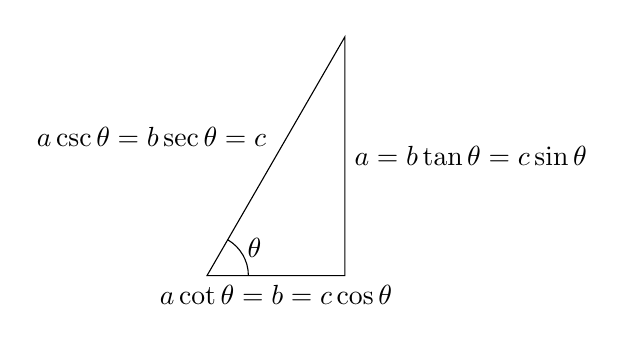
\begin{tikzpicture}[scale=1.75]
		\node (A) at (0,0) {};
		\node (C) at (1,0) {};
		\node (B) at (60:2) {};
		\draw (A.center) -- node[above left]{$a \csc\theta = b \sec\theta = c$} (B.center) -- node[right]{$a = b \tan\theta = c \sin\theta$} (C.center) -- node[below]{$a \cot\theta = b = c \cos\theta$} cycle;
		\draw (.3,0) arc (0:60:.3) node[pos=.7,right]{$\theta$};
	\end{tikzpicture}
	\caption{Razones trigonométricas}\label{fig:trig-functions}
\end{figure}
\begin{prop}
Sea $\theta$ un ángulo cualquiera, se cumple que:
	\begin{align}
		\sin^2\theta+\cos^2\theta&=1,\\
		1+\tan^2\theta&=\sec^2\theta,\\
		1+\cot^2\theta&=\csc^2\theta.
	\end{align}
\end{prop}
Ahora introduciremos la analogía del círculo unitario o goniométrico. Consideremos una recta $r$, un punto $O \in r$ y otro $C \in r$ tal que dada una métrica aditiva lineal $\mu$ se cumpla que $\mu(\overline{OC}) = 1$, construimos una $\omega$ con centro $O$ y radio $\overline{OC}$. Luego, con un semiplano que contenga a $\omega$, de frontera $r$ y con la semirrecta $\overrightarrow{OC}$ construimos el ángulo $\theta$ y por ende $A$ como la intersección de su lado restante con $\omega$ (que se intersecta en un único punto), definimos a $B$ como el pie de la perpendicular a $r$ por $A$ y a $D$ como la intersección entre la perpendicular a $r$ por $C$ y $OA$. En este caso se da
que:
$$\sin(\theta)=\frac{\overline{CD}}{\overline{OD}}=\mu(\overline{AB}),\; \cos(\theta)=\frac{\overline{OC}}{\overline{OD}}=\mu(\overline{OB}),\; \tan(\theta)=\frac{\overline{AB}}{\overline{OB}}=\mu(\overline{CD}).$$
\begin{figure}
	\centering
	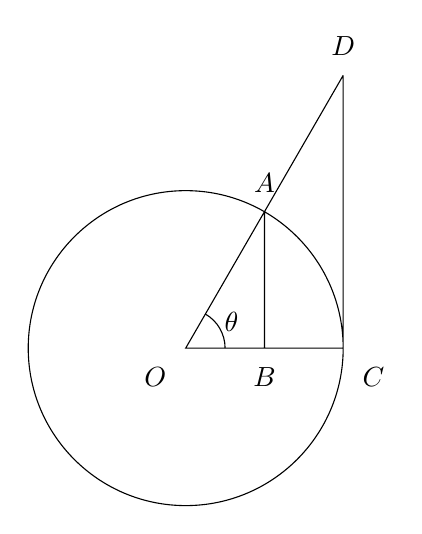
\begin{tikzpicture}[scale=2]
		\node[label=below left:{$O$}] (O) at (0,0) {};
		\node[label=above:{$A$}] (A) at (60:1) {};
		\node[label=below:{$B$}] (B) at (.5,0) {};
		\node[label=below right:{$C$}] (C) at (1,0) {};
		\node[label=above:{$D$}] (D) at (60:2) {};
		\draw (O) circle (1) (D.center) -- (O.center) -- (C.center) -- (D.center) (A.center) -- (B.center);
		\draw (.25,0) arc (0:60:.25) node[pos=.7,right]{$\theta$};
	\end{tikzpicture}
	\caption{}
\end{figure}
\begin{thm}[Teorema del coseno]\index{teorema!del coseno}
	Todo triángulo $\triangle ABC$ satisface la siguiente ecuación:
	\begin{equation}
		a^2=b^2-2bc\cos(\angle A)+c^2
	\end{equation}
\end{thm}
\begin{proof}
	Comenzamos por definir $D$ como el pie de la perpendicular a $AB$ por $C$, luego llamaremos $h := \overline{CD}$, $c_1 := \overline{AD}$ y $c_2 := \overline{DB}$, de forma que, por teorema de Pitágoras, tendremos las siguientes ecuaciones:
	$$b^2=c_1^2+h^2,\quad a^2=h^2+c_2^2$$
Despejando $h$ y reemplazando en la ecuación de a nos queda:
	$$a^2=b^2+c_2^2-c_1^2=b^2+(c_1+c_2)(c_2-c_1)$$
Ahora, dividiremos los casos según si $\theta$ es agudo u obtuso (pues, de ser recto, el teorema estaría probado).
	\begin{figure}
		\centering
		\begin{tikzpicture}[scale=2]
			\node[label=below left:{$A$}] (A) at (0,0) {};
			\node[label=below:{$B$}] (B) at (1,0) {};
			\node[label=above right:{$C$}] (C) at (2,1) {};
			\node[label=below:{$D$}] (D) at (2,0) {};
			\draw (A.center) -- (B.center) -- (C.center) -- cycle;
			\draw[dashed] (B.center) -- (D.center) -- (C.center);
			\draw (.4,0) arc (0:30:.4) node[pos=.7,right]{$\theta$};
		\end{tikzpicture}
		\caption{}
	\end{figure}

Trataremos el caso en que $\theta$ es agudo. Considere que $c_1 = b \cos \theta$. Luego se puede dar que $\angle B$ sea agudo o obtuso. Si es agudo, entonces $c = c_1 + c_2$, de forma que queda instantáneamente probado. Si es obtuso, entonces $c = c_1-c_2$, con lo que
	\begin{align*}
		a^2&=b^2+(c+2c_2)(-c)=b^2-c^2-2cc_2\\
		&=b^2+c^2-2c(c+c_2)=b^2-2bc\cos\theta+c^2.
	\end{align*}
Si $\theta$ es obtuso, por definición $c_1 = b \cos(\pi - \theta) = -b \cos \theta$ y $c = c_2 - c_1$, por lo que
	$$a^2=b^2+(c-2c_1)c=b^2+2bc\cos\theta+c^2$$
como se quería probar.
\end{proof}
Nótese que el teorema del coseno puede considerarse una generalización del teorema de Pitágoras.
\begin{thm}[Circuncentro y circunradio]
	Dado un triángulo $\triangle ABC$ llamaremos \textit{circunferencia circunscrita}\index{circunferencia!circunscrita} a aquella $\omega$ coplanar a ella, tal que $A,B,C\in\omega$. Al centro de esta circunferencia le decimos su \textit{circuncentro}\index{circuncentro} al centro de esta circunferencia y su \textit{circunradio}\index{circunradio} al radio de ésta.
\end{thm}
\begin{prop}
En un triángulo, su circuncentro es la intersección de sus mediatrices.
\end{prop}
\begin{proof}
	Denotemos $m_a$ la mediatriz de $a$, y así para el resto. Nótese que para todo $P\in m_a$ se cumple que $\overline{PB}\equiv\overline{PC}$ (pues si $A'$ es el punto medio de $a$, entonces $\triangle PA'B\equiv\triangle PA'C$ por LAL) y así para el resto de lados. Entonces, definamos $O$ como la intersección de $m_a$ y $m_b$, por lo que, $\overline{OA}\equiv\overline{OB}\equiv\overline{OC}$, luego, $O\in m_c$.
\end{proof}
\begin{thm}[Teorema del seno]\index{teorema!del seno}
Todo triángulo $\triangle ABC$ de circunradio $R$ satisface la siguiente ecuación:
	\begin{equation}
		\frac{a}{\sin(\angle A)}=\frac{b}{\sin(\angle B)}=\frac{c}{\sin(\angle C)}=2R
	\end{equation}
\end{thm}
\begin{proof}
Sea $D$ el pie de la perpendicular a $AB$ por $C$. Entonces, se cumple que:
$$CD \equiv a \sin(\angle B) \equiv b \sin(\angle A),$$
	por ende, la relación buscada. Sea $O$ el cicumradio de la circunferencia y sea $E$ el punto tal que $\overline{EC}$ es un diámetro. Luego, en el triángulo $\triangle EBC$ podemos aplicar la relación enseñada:
	$$\frac{a}{\sin(\angle A)}=\frac{e}{\sin(\angle E)}=\frac{2R}{\sin(\angle EBC)}=2R$$
Esto puesto que $a \equiv e$, $\angle A \equiv \angle E$ (pues abarcan el mismo arco y están inscritos en la circunferencia) y que $\angle EBC \equiv \pi/2$ (debido a que está inscrito en la circunferencia y abarca una semicircunferencia).
\end{proof}

\section{Geometría de triángulos}
\begin{mydef}
	Dado un triángulo $\triangle ABC$ y un segmento $\overline{AB}$ que llamaremos \textit{base}, entonces llamaremos su \textit{altura}\index{altura} a la recta perpendicular a la base que pasa por el punto restante (es decir, $C$ en este caso). Asimismo llamaremos el \textit{pie}\index{pie!(de la altura)} de la altura a la intersección $P_c$ entre la altura y la base y admitiremos el convenio de denotar $h_c$\nomenclature{$h_a$}{Altura (segmento) del lado $a$ de un triángulo.} al segmento $\overline{CP_c}$.

	Dado un vértice (i.e. $A$), llamaremos \textit{mediana}\index{mediana} a la recta que pasa por dicho punto y el punto medio del lado opuesto (en este caso, $\overline{BC}$).

	Más generalmente, llamaremos \textit{cevianas}\index{ceviana} a todo segmento que emerge desde un vértice del triángulo e intersecta a la prolongación del segmento opuesto. En este caso, las bisectrices, alturas y medianas son, en efecto, cevianas.
\end{mydef}
\begin{thm}
Las alturas de un triángulo son inversamente proporcionales a las bases del mismo resp. Es decir,
	$$\frac{h_a}{h_b}=\frac{b}{a}.$$
\end{thm}
\begin{proof}
	Sean $P$, $Q$ los pies de las alturas de $a,b$ resp., entonces $P$ es colineal con $B,C$ y $Q$ con $A,C$, de forma que $\angle PCA\equiv\angle BCA \equiv\angle BCQ$. Luego, $\triangle APC\sim\triangle BQC$ (pues comparten un ángulo recto), por ende se concluye la relación.
\end{proof}
\begin{mydef}[Área]
	Dada una medida lineal $m$, diremos que la función área derivada $\alpha_m$ es aquella de dominio los triángulos de un espacio y codominio $\R$ tal que si un triángulo $\triangle$ posee base $b$ y altura $h$, el área es
	$$\alpha(\triangle)=\frac 12m(b)m(h).$$
	Asimismo, definimos que
	$$\alpha(\triangle_1 \cup \triangle_2)= \alpha\triangle_1 + \alpha\triangle_2 - \alpha(\triangle_1\cap\triangle_2)$$
\end{mydef}
En general, a menos que se utilice una medida específica se obviará el subíndice, de forma que se escriba $\alpha$ a secas para representar el área.
\begin{prop}
	Sean $\triangle_1,\triangle_2$ triángulos, entonces:
	\begin{enumerate}
		\item $\triangle_1\equiv\triangle_2$ implica $\alpha\triangle_1=\alpha\triangle_2$.
		\item El área de cualquier segmento, punto, o conjunto finito de ambos es nulo.
	\end{enumerate}
\end{prop}
\begin{mydef}[Polígono]
	Diremos que dos triángulos son \textit{contiguos} cuando su intersección corresponde a un conjunto de segmentos o puntos. Llamaremos \textit{polígono}\index{polígono} a la figura formada por la unión de finitos triángulos contiguos y coplanares. Trivialmente, resulta que los triángulos y paralelogramos son polígonos.
\end{mydef}
Nótese que bajo nuestras definiciones, sólo se puede calcular el área de polígonos. Por ello, realizaremos una generalización:
\begin{mydef}[Área (def. de Jordan)]
	Sea $A$ un subconjunto de un plano, entonces definimos su área interior y exterior resp. como
	\begin{align}
		\underline{\alpha}A&=\sup\left\{\sum_{i=1}^\infty\alpha P_i:P_i\text{ polígono}\wegde\bigcup_{i=1}^\infty P_i\subseteq A\right\}\\
		\overline{\alpha}A&=\inf\left\{\sum_{i=1}^\infty\alpha P_i:P_i\text{ polígono}\wegde\bigcup_{i=1}^\infty P_i\supseteq A\right\}.
	\end{align}
	Diremos, finalmente, que $A$ es medible y posee área $\alpha A=\underline{\alpha}A=\overline{\alpha}A$.
\end{mydef}
Es evidente que todo polígono conserva su área, 

Diremos que una proporción posee las \textit{longitudes dirigidas} cuando, dados $A,B,C,D$ colineales, la cantidad
$$\frac{\overline{AB}}{\overline{CD}}$$
es positiva si $ {<_{AB}} = {<_{CD}} $ y negativa de lo contrario.
\begin{thm}[Teorema de Ceva]\index{teorema!de Ceva}
	En un triángulo $\triangle ABC$ se cumple que las cevianas $\overline{AD}, \overline{BE}, \overline{CF}$ son concurrentes syss
	$$\frac{\overline{AD}}{\overline{DB}} \frac{\overline{BE}}{\overline{EC}} \frac{\overline{CF}}{\overline{FA}}=1$$
	con las longitudes dirigidas.
\end{thm}
\begin{proof}
$\implies$. Digamos que se intersectan en $P$, entonces, es inmediata las relaciones:
	$$\frac{\overline{BD}}{\overline{DC}}=\frac{\alpha\triangle BAD}{\alpha\triangle DAC}=\frac{\alpha\triangle BPD}{\alpha\triangle DPC},$$
	algebraicamente, $\frac{a}{b}=\frac{x}{y}=\frac{a+x}{b+y}$, por lo que, resulta
	$$\frac{\overline{BD}}{\overline{DC}}=\frac{\alpha\triangle BAD-\alpha\triangle BPD}{\alpha\triangle DAC-\alpha\triangle DPC}=\frac{\alpha\triangle APB}{\alpha\triangle APC}.$$
	De manera análoga, se comprueba que
	$$\frac{\overline{CE}}{\overline{EA}}=\frac{\alpha\triangle BPC}{\alpha\triangle APB},\quad\frac{\overline{AF}}{\overline{FB}}=\frac{\alpha\triangle APC}{\alpha\triangle BPB}$$
	Con lo que obtenemos la ecuación deseada.
$\Longleftarrow$. Digamos que las cevianas $\overline{BE}, \overline{CF}$ se intersectan en $P$, tal que definimos $ \overline{AD'} $ como la ceviana que pasa por $P$ y que, por ende, satisface la ecuación descrita. Despejando ambas ecuaciones obtenemos que
	$$\frac{\overline{BD}}{\overline{DC}}=\frac{\overline{BD'}}{\overline{D'C}},$$
	de lo que se concluye inmediatamente que $D=D'$.
\end{proof}
\begin{thm}[Teorema de Menelao]\index{teorema!de Menelao}
	Dado un triángulo $\triangle ABC$, tal que los puntos $D,E,F$ pertenecen a las rectas $AB,BC,CA$ resp., entonces dichos puntos son colineales syss
	$$\frac{\overline{AD}}{\overline{DB}} \frac{\overline{BE}}{\overline{EC}} \frac{\overline{CF}}{\overline{FA}}=-1$$
	con las longitudes dirigidas.
\end{thm}
\begin{proof}
	$\implies$. Nótese que el convenio de signos se deduce de forma inmediata mediante el axioma y el primer teorema de Pasch. Cabe destacar que las demostraciones no varían si los puntos son externos o si dos de ellos son internos.

	Como son colineales llamemos $r=DF$ y $H_A$ al pie de la perpendicular a $r$ por $A$ (y así con el resto). Lo siguiente lo separaremos en dos casos: $r$ es o no perpendicular a algún lado del triángulo. En el primer caso, sin perdida de generalidad supondremos que es perpendicular a $BC$. Luego, $BC\parallel AH_A$, con lo que podemos concluir con facilidad que $\triangle AH_AD\sim\triangle BED$ y que $\triangle AH_AF\sim\triangle CEF$, por ende,
	$$\frac{\overline{AD}}{\overline{BD}}=\frac{\overline{AH_A}}{\overline{BE}},\quad\frac{\overline{CF}}{\overline{FA}}=\frac{\overline{EC}}{\overline{AH_A}}$$
	con lo cuál queda resuelta la demostración para este caso.

	Para el segundo caso, sin perdida de generalidad, supondremos que $r$ no intersecta a $\overline{AB}$. Luego, se demuestra que $\triangle BEH_B\sim\triangle CEH_C$ y que $\triangle AFH_A\sim\triangle CFH_C$ (por poseer un ángulo recto y por ángulos opuestos por el vértice), además que $\triangle AH_AD\sim\triangle BH_BD$, con lo que, nuevamente se completa el enunciado con una aplicación del teorema de Tales.
	
	La coimplicancia es análoga al caso con el teorema de Ceva.
\end{proof}
\begin{lem}
En $\triangle ABC$ con $M_a$ el punto medio de $a$, se cumple que $M_aM_b\parallel AB$.
\end{lem}
\begin{proof}
Veamos que $\triangle ABC\sim\triangle AM_aM_b$, por lo que $\angle B\equiv \angle AM_bM_a$ y $\angle C\equiv\angle AM_aM_b$. Finalmente, como los ángulos internos son congruentes, las rectas son paralelas.
\end{proof}
\begin{thm}
	Las medianas de un triángulo son concurrentes, y llamaremos a dicho punto \textit{baricentro} o \textit{centroide}\index{baricentro, centroide} y le denotaremos con la letra $G$. El baricentro divide al triángulo en seis triángulos de áreas iguales y divide a las medianas en la razón $2:1$. 
\end{thm}
\begin{proof}
	La concurrencia es inmediata del teorema de Ceva.

	Para el resto, denotemos $M_a$ el punto medio de $a$, de forma que trivialmente se concluye que $x:=AGM_c=M_cGB$, $y:=AGM_b=M_bGC$ y $z:=BGM_a=M_aGC$ (ver fig.~\ref{fig:triangle-s-centroid}). Asimismo, $x+2y=ACM_c=M_cCB=x+2z$, de lo que se concluye que $y=z$ y análogamente para ver que $x=y$.
\begin{figure}
	\centering
	\begin{tikzpicture}
		\node[label=below left:{$A$}] (A) at (0,0) {};
		\node[label=below right:{$B$}] (B) at (5.5,0) {};
		\node[label=above:{$C$}] (C) at (2,3) {};
		\node (ma) at (3.75,1.5) {};
		\node (mb) at (1,1.5) {};
		\node (mc) at (2.75,0) {};
		\node (G) at (2.5,1) {};
		\fill[niceblue!75] (A.center) -- (G.center) -- (B.center) -- cycle;
		\fill[nicegreen!75] (C.center) -- (G.center) -- (B.center) -- cycle;
		\fill[nicered!75] (A.center) -- (G.center) -- (C.center) -- cycle;
		\draw (A.center) -- node[sloped]{$\shortmid$} (mc.center) -- node[sloped]{$\shortmid$} (B.center) -- node[sloped]{$\shortparallel$} (ma.center) -- node[sloped]{$\shortparallel$} (C.center) -- node[sloped]{$\shortparallel\shortmid$} (mb.center) -- node[sloped]{$\shortparallel\shortmid$} (A.center);
		\draw (A.center) -- (ma.center) (B.center) -- (mb.center) (C.center) -- (mc.center);
	\end{tikzpicture}
	\caption{}\label{fig:triangle-s-centroid}
\end{figure}

	La última demostración es la más complicada de todas. Primero, definamos $\ell:=\overline{CM_c}$ y
	$$r:=\frac{\overline{CG}}{\overline{CM_c}},$$
	o, lo que es equivalente, que $\overline{GM_c}\equiv(1-r)\ell$.

	Luego, definamos $M_c^{\prime}$ como la intersección entre $M_aM_b$ y $CM_c$. Por teorema de Tales, se concluye que $\overline{CM_c^{\prime}}\equiv\ell/2$. Por el lema anterior, concluimos que $\triangle ABC\sim\triangle  M_aM_bM_c$ y por Tales es también inmediato concluir que $M_c^{\prime}$ es punto medio de $\overline{M_aM_b}$, que $ \overline{M_cM_c^{\prime}} \equiv\ell/2$ y que, por lo tanto (y considerando que $\triangle ABC$ y $\triangle M_aM_bM_c$ comparten baricentro), $\overline{GM_c} \equiv r\ell/2$. Finalmente, por álgebra concluimos que $r=2/3$, por lo que los segmentos $\overline{CG}:\overline{GM_c}$ están a razón $2:1$ como dijimos.
\end{proof}
\begin{thm}
	Las alturas de un triángulo son concurrentes y llamaremos a su intersección \textit{ortocentro}\index{ortocentro} y le denotaremos con la letra $H$\nomenclature{$H$}{Ortocentro}.
\end{thm}
\begin{thm}
	En un triángulo cualquiera el circuncentro, baricentro y ortocentro son colineales, llamamos a esta recta la \textit{recta de Euler}\index{recta!de Euler}. Además $\overline{HG}:\overline{GO}$ están en razón $2:1$.
\end{thm}
\begin{proof}
	Dado $\triangle ABC$, igual que con las medianas, admitamos que $M_a$ es el punto medio de $a$. Definamos $H'$ como la intersección entre $OG$ con $h_a$, de forma que $\triangle AGH'\sim\triangle M_aGO$. Definamos también $H''$ como la intersección entre $OG$ con $h_b$, de forma que $\triangle BGH''\sim\triangle M_bGO$.

	Nótese que por el teorema anterior, sabemos que $\overline{AG}:\overline{GM_a}=\overline{BG}:\overline{GM_b}=2:1$, por lo que, $\overline{H'G}\equiv2\overline{GO}\equiv\overline{H''G}$, de lo que se concluye que $H'=H''$ y que es, efectivamente, el ortocentro del triángulo.
\end{proof}

\subsection*{Cálculo de áreas}
\begin{thm}
	Dado $\triangle ABC$ de semiperímetro $s:=\frac{a+b+c}{2}$ y circunradio $R$ entonces
	$$\alpha(\triangle ABC)=\frac{abc}{4R}=\sqrt{s(s-a)(s-b)(s-c)}$$
	(la segunda fórmula es llamada la \textit{fórmula de Herón}\index{fórmula de Herón}).
\end{thm}
<++>
\begin{thm}
Un paralelogramo de base $b$ y altura $h$ posee un área de $bh$.
\end{thm}
<++>
\begin{thm}
	Una sección de un círculo de radio $r$ que abarca $\theta$ de arco es medible y posee un área de $\frac{1}{2}\theta r^2$. En particular, el área de dicho círculo es $\pi r^2$.
\end{thm}
\begin{proof}
	Para esta demostración utilizaremos métodos propios del análisis matemático, por ende, puede que no todo lector sea capaz de seguirnos. Dado $\theta=\overarc{AB}$, definiremos $A_1,\dots,A_{2^N}$ tal que $A=A_0$, $A_{2^n}=B$ y $\overarc{A_0A_1}=\overarc{A_1A_2}=\cdots=\overarc{A_{2^n-1}A_{2^n}}$. Sea $O$ el centro del círculo, entonces
	$$P_n:=\bigcup_{k=0}^{2^n}\triangle OA_kA_{k+1}$$
	Asimismo, dado $0\leq k< 2^n$ cualquiera, entonces consideramos la intersección entre la bisectriz de $\angle A_kOA_{k+1}$ y a circunferencia, para luego construir la perpendicular $r$ a ella y finalmente definir $B_k$ como la intersección entre $r$ y $OA_k$, y hacer lo mismo con $B_{k+1}$, de forma que definimos
	$$P_n^{\prime}:=\bigcup_{k=0}^{2^n}\triangle OB_kB_{k+1}$$
	\begin{figure}
		\centering
		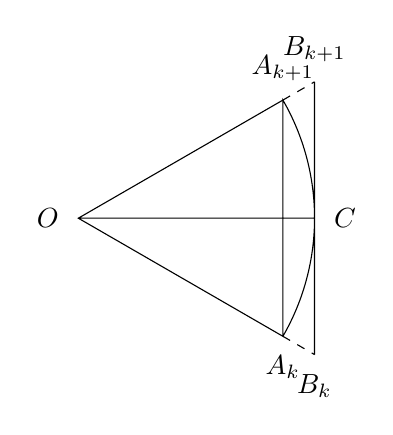
\begin{tikzpicture}
			\node[label=left:{$O$}] (O) at (0,0) {};
			\node[label=above:{$A_{k+1}$}] (A1) at (30:3) {};
			\node[label=below:{$A_k$}] (A2) at (-30:3) {};
			\node[label=above:{$B_{k+1}$}] (B1) at (30:{3*sec(30)}) {};
			\node[label=below:{$B_k$}] (B2) at (-30:{3*sec(30)}) {};
			\node[label=right:{$C$}] (C) at (3,0) {};
			\draw (A1.center) -- (O.center) -- (A2.center) -- (A1.center) arc (30:-30:3) (O.center) -- (C.center) (B1.center) -- (B2.center);
			\draw[dashed] (A1.center) -- (B1.center) (A2.center) -- (B2.center);
		\end{tikzpicture}
		\caption{}
	\end{figure}

	Está más que claro que si $\mathcal{C}$ es la sección que buscamos, $P_n\subseteq\mathcal{C}\subseteq P_n^{\prime}$. Y es fácil comprobar que las áreas están dadas por las fórmulas:
	\begin{align}
		P_n&=2^nr^2\sin\left(\frac{\theta}{2^{n+1}}\right)\cos\left(\frac{\theta}{2^{n+1}}\right)=\frac{\theta r^2}{2}\frac{2^n}{\theta}\sin\left(\frac{\theta}{2^n}{\right),\\
		P_n^\prime&=2^{n+1}r^2\tan\left(\frac{\theta}{2^{n+1}}\right)=\frac{\theta r^2}{2}\frac{2^{n+1}}{\theta}\tan\left(\frac{\theta}{2^{n+1}}{\right).
	\end{align}
	Nótese que los términos derechos (los que dependen de $n$ por si acaso) convergen a 1 (utilizando límites de funciones estudiadas en el libro de Análisis), por ende, por definición se obtiene que el área es $\theta r^2/2$, es decir, que el área de un círculo es $\pi r^2$.
\end{proof}

\section{Geometría analítica}
Mediante la geometría sintética (es decir, la que ya hemos analizado en los capítulos previos) hemos obtenido una gran cantidad de resultados muy potentes, sin embargo, los matemáticos pronto se darían cuenta de que no es sino hasta que las ramas de las matemáticas se conectan que éstas alcanzan su máximo potencial y se diversifican dando a lugar a las ideas más brillantes y complejas que la humanidad es capaz de otorgar. Descartes es, en esta narrativa, el héroe que plantea por primera vez una perspectiva analítica y algebraica de la geometría. Cabe destacar que los métodos de este capítulo son, aún básicos para lo que representan ambas materias en la actualidad, no obstante, se recomienda y requiere un conocimiento elemental en ambas (especialmente todo lo correspondiente al \textit{álgebra lineal} pues es el punto fuerte del capítulo).

\section{Vectores}
\begin{mydef}[Recta dirigida]
	Dada una recta $r$ y un ordenamiento $<$, llamaremos al par $(r,<)$ una \textit{recta dirigida}\index{recta!dirigida}. Dada otra recta dirigida $(s,<')$, diremos que poseen la misma orientación o dirección syss es paralela a $r$ y si dada una recta $t$ secante a $r$, y a $s$, cortándoles en $P$ y $P'$ resp., entonces los puntos mayores a cada recta son coplanares respecto a $t$.
\end{mydef}
\begin{lem}
La propiedad entre rectas de poseer la misma orientación o dirección corresponde a una relación de equivalencia.
\end{lem}
\begin{proof}
La reflexividad y simetría son triviales. 
\end{proof}
\begin{mydef}[Vectores]
	Diremos que $\overrightarrow{AB}=(\mu(\overline{AB}), [AB,<_{AB}])$\nomenclature{$\overrightarrow{AB}$}{Vector de $A$ a $B$.} es un \textit{vector}\index{vector}. Asimismo, definimos el \textit{módulo}\index{modulo@módulo!de un vector} de dicho vector al valor $\|\overrightarrow{AB}\|:=\mu(\overline{AB})$; cabe descatar que la función $\|\,\|$ se le llama \textit{norma}\index{norma} del espacio. Asimismo, llamamos a la recta dirigida $(AB,<_{AB})$ su prolongación. También diremos que los puntos $A,B$ son el origen y el extremo resp. del vector. En caso de que el origen sea igual al extremo, consideramos que su módulo es nulo y carece de dirección, por ende, se puede representar simplemente por el número cero o un conjunto que sólo le contiene.

	Observe que dos vectores son iguales syss poseen el mismo módulo (poseen igual medida) y sus prolongaciones comparten dirección, su cualidad de iguales no depende de sus extremos. Esta idea de ser una cantidad con dirección representa la idea fundamental de ellos.
\end{mydef}
En este contexto, el axioma IV2 puede replantearse como que dada un vector $\vec{v}$ y un punto $P$, sólo existe un punto $Q$ tal que $\overrightarrow{PQ}=\vec{v}$ y así le utilizaremos a lo largo de este capítulo.

Dado un punto cualquiera, digamos $O$ se puede formar $V$ como el conjunto de todos los vectores de la forma $\overrightarrow{OP}$ con $P$ un punto cualquiera del espacio. Por lo ya dicho anteriormente, este conjunto es independiente de la elección de $O$; y le denotaremos como $V$.

Ahora, veremos dos posibles ``acciones'' (que son funciones que representan operaciones): la primera, la llamaremos la \textit{multiplicación} o \textit{producto por un escalar}. Sea $R$ el conjunto de todos los posibles números derivados de las proporciones entre segmentos de un espacio --que sabemos es un subconjunto de los reales y superconjunto de los racionales--, y sea $\alpha\in R$, entonces $\alpha\vec{v}$ será el vector nulo si $\alpha$ lo es, de lo contrario será el vector de módulo $|\alpha|\,\|\vec{v}\|$ con dirección\footnote{Aquí $\sign\alpha$ es la función que otorga el signo de $\alpha$. Otra observación es que, si bien la notación puede ser poco convencional, realmente no es nada del otro mundo. ${<^{+1}}={<}$ y ${<^{-1}}={>}$.} $(r,<^{\sign\alpha})$ (donde $(r,<)$ corresponde a la orientación de $\vec{v}$). La segunda, es la \textit{adición de vectores}. En particular, la operación $\vec{u}+\vec{v}$ define el vector resultante de la siguiente construcción: se comienza eligiendo un punto $O$ cualquiera, luego existe un único $P$ tal que $\overrightarrow{OP}=\vec{u}$ y existe un único $Q$ tal que $\overrightarrow{PQ}=\vec{v}$; finalmente, $\vec{u}+\vec{v}:=\overrightarrow{OQ}$.

Cabe destacarse también que la ecuación $\overrightarrow{PQ}=\vec v$ se verá en ocasiones descrita como que $Q=P+\vec v$.
\begin{thm}
	$(V,+,\cdot)$ es un $R$-espacio vectorial de dimensión 3.
\end{thm}
\begin{proof}
	Primero se requiere probar que $(V,+)$ es un grupo abeliano. La conmutatividad, elemento neutro e inversos son triviales (para la primera usar las propiedades del paralelogramo). Con la construcción utilizada en la definición de suma es también sencillo comprobar la transitividad.

	Respecto a la operación externa (es decir, el producto por un escalar). Siendo $u,v\in V$ y $x,y\in R$ las propiedades $1v=v$ y $x(yv)=(xy)v$ son triviales. La propiedad $x(u+v)=xu+xv$ se comprueba por teorema de Tales y $(x+y)v=xv+yv$ se comprobó al definir la proporcionalidad.
\end{proof}
Es aquí cuando se hace tangible la conexión de la que nos jactabamos al iniciar el capítulo. 

Para empezar, conviene introducir la noción algebraica de \textit{independencia lineal}\index{linealmente!independientes (vectores)}. En ella, un conjunto de vectores $v_1,\dots,v_n\in V$ se le considera como tal syss la ecuación
$$\sum_{i=1}^n\lambda_n v_n=0$$
es verdad sólo con $\lambda_k=0$ para todo $1\leq k\leq n$ natural.

De esto, es trivial ver que dos vectores son linealmente independientes syss dado un punto $P$ cualquiera, los puntos $P$, $P+\vec v$ y $P+\vec u$ no son colineales.
\begin{thm}

\end{thm}
<++>

\part*{Apéndices}
\appendix
\chapter{Biografías matemáticas}
Los matemáticos que hemos de describir acontinuación corresponden a un grupo selecto de los más importantes para la misma, luego, no será de extrañar que si ha leído alguna de sus biografías, se encontrará con una falta absoluta de detalles que, me veo obligado a justificar; el objetivo de este capítulo es el de dar una introducción o una vaga idea de quiénes son tales personajes, su lectura a detalle es altamente recomendada, que lo disfrute.

\section{Pitágoras}
$\Pi\upsilon\theta\alpha\gamma\acute{o}\rho\alpha\varsigma$, más conocido como \textit{Pitágoras de Samos}, nació alrededor de 569 A.C. en Samos, Jonia (actualmente Grecia). Era hijo de un mercader de Tiro (actualmente en Líbano) quien le hacía acompañarle durante sus abundantes viajes que incluyen Tiro, Siria e Italia.

Poco se sabe de la infancia de Pitágoras, mas hay registros de que tocaba la lira y recitaba Poesía, Homero en particular. Además, se sabe haber conocido a tres filósofos cuya influencia es de alta relevancia para el joven griego, Ferécides de Siros, Tales de Mileto y su pupilo Anaximandro. Los cuales les enseñaron sobre matemáticas --con énfasis en la geometría-- y cosmología.

Al rededor de 535 A.C. Pitágoras fue a Egipto por una carta de Polícrates, tirano de Samos en aquél entonces. Según Porfirio, Pitágoras habría aprendido bastante de geometría con los Egipcios, mas no se duda acerca de la influencia de Tales y Anaximandro. Cerca de 525 A.C. Cambises II, rey de Persia, invade Egipto y capturan a Pitágoras enviándolo a Babilonia. Cerca de 525 A.C. Polícrates y Cambises II mueren (se sospecha que por accidente o suicidio) y en 520 A.C. Pitágoras es liberado y retorna a Samos, no se sabe si la muerte de ellos fuese un factor en esto último.

En Samos intenta establecer una escuela llamada ``el semicírculo'', pero dos años más tarde abandona el proyecto y se traslada a Croton (actualmente Crotona, Italia) donde estable su escuela pitagórica para fomentar el pensamiento crítico matemático y ético-filosófico. Otro detalle a destacar es que su establecimiento admite tanto a hombres como mujeres. De las lecciones partículares no hay registro formal, mas se sabe que fomenta principalmente las metamatemáticas (como la discusión del concepto de número, de triángulo, etc.), la teoría de números (principalmente números triangulares y perfectos) y geometría. Hay varios teoremas conocidos asociados a los pitagóricos, mas, ironicamente, el teorema de Pitágoras fue descubierto y demostrado mucho ántes del personaje (al menos un milenio ántes de hecho).

Pitágoras muere cerca del 475 A.C. en Metaponto, Italia.

\section{Euclides}
$E\upsilon\kappa\lambda\varepsilon\acute{\iota}\delta\eta\varsigma$, más conocido como \textit{Euclides de Alexandría}, 

\section{David Hilbert}
\begin{wrapfigure}{R}{.3\textwidth}
\centering
\includegraphics[width=.275\textwidth]{Hilbert.jpg}
\caption{Hilbert en 1912.}
\end{wrapfigure}

David Hilbert, nacido el 23 de enero de 1862 en Königsberg, Prusia es lo que a las matemáticas modernas y formales, lo que Mozart al clasicismo. Y es que invocando el nombre de tan legítimo músico pretendo establecer más que un simple paralelo, pues ambos nacieron \textit{hechos} para lo que fueron. La madre del joven Hilbert era amante de las matemáticas --en particular, de la teoría de números--, su familia la describen como acomodada y la ciudad es caracterizada por el problema de los siete puentes (resuelto por \textbf{L. Euler}) y los matemáticos nacidos allí como \textbf{I. Kant} y \textbf{C. Goldbach}; llegada su adultez, David se inscribió en la Universidad de Köningsberg a estudiar matemáticas --en contra de su padre que quería que estudiase leyes--.

Aquella universidad sería crucial para la vida del matemático, pues su libertad para tomar lecturas, charlas y cursos le llevarían a conocer en detalle el mundo de las matemáticas contemporáneas. Además de ello, conocería a sus dos más grandes y cercanos amigos, Hermann Minkowski y Adolf Hurwitz, de los que recibiría halagos al entregar su tesis doctoral sobre la teoría de invariantes algebraicas.

Tras su doctorado comenzó a trabajar en su post-doctorado o \textit{Habilitation}, y más tarde en el título de Profesor \textit{Extraordinarius}, recibiendo clases de \textbf{F. Klein} --quién pretende ser el Riemann de la época--. A sugerencia de su profesor --quién luego se convertiría en su amigo--, él viaja a Paris a conocer en persona a los grandes matemáticos, entre ellos, a \textbf{Hermite} quién le introduce al \textit{problema de Gordan}, el cual le valdría de inmensa popularidad al matemático, en especial por su generalidad al aplicarse a distintos campos como la geometría algebraica o la teoría de números.

En la vida personal se le describe como una persona sociable, que casualmente visitaba bailes y fiestas y hacía de su hogar un colectivo de colegas. Es gracias a esta característica suya de la que conoce a Käthe Jerosh, prima segunda suya, con la que contrae matrimonio que da lugar a su único hijo Franz.

Además de compararle con Mozart, diría que es a las matemáticas lo que Feynman es a la física. Y este último aspecto lo hago para adelantar el hecho de que se le reconoce en su entorno como un hombre cuyas lecturas eran arduamente inspiradoras, al punto de que su Instituto de Göttingen es famoso por admitir a matemáticos como \textbf{H. Weyl}, \textbf{E. Lasker} (campeón mundial de ajedrez), \textbf{E. Zermelo} y \textbf{C. Hempel}. Además de constar de un grupo social conformado por figuras como \textbf{von Neumann}, \textbf{E. Noether} y \textbf{A. Church}. Debido al crecimiento del movimiento nazi se termina por desinstaurar este templo del saber, ante la duda del ministro de educación al respecto, Hilbert responde: \textit{``Ya no existen las matemáticas en Göttingen''}.

Durante su vida Hilbert demuestra un profundo interés sobre la formalización de las matemáticas, la idea de la construcción absoluta de ella sobre los pilares que son los axiomas, de hecho, en el año 1900 publica su famosa lista de \textit{los 23 problemas de Hilbert}, la mayoría tratando los temas de consistencia y propiedades contemporáneas únicas a las teorías más modernas y precisas como la trascendencia irracional o la cardinalidad infinita, esto concuerda con que el hombre vivió durante la \textbf{crisis fundacional de las matemáticas} --el problema \textit{¿de dónde viene la matemática?}--. Más tarde daría charlas sobre su reformulación de la geometría euclidea (ver capítulo~1) y la fundación de la teoría algebraica de números.

Hilbert muere en Göttingen a la edad de 81 años el 14 de febrero de 1943.

\textit{``Debemos saber y sabremos''.}

\printindex
\printnomenclature

\nocite{*}
\printbibliography[heading=bibintoc]

\end{document}
